\chapter{Despliegue y Operación}\label{cap:sum}

\section{Introducción}
Este capítulo aborda el proceso integral de instalación y puesta en marcha del servicio, detallando el despliegue de la pila de contenedores en Swarm. Además, se proporciona una guía práctica sobre el uso efectivo de la misma.


\section{Instalación de la Plataforma}

Para iniciar el proceso de instalación, es necesario contar con el repositorio de deploy. Puede clonar el repositorio desde GitHub utilizando el siguiente comando:


%estilo de comando
\lstdefinestyle{consola} {
    numbers=none,
    xleftmargin=\parindent,
    xrightmargin=\parindent,
    aboveskip=3mm,
    belowskip=0.01mm,
    basicstyle=\small\bf\ttfamily,
    backgroundcolor=\color{black!08},
}


\begin{lstlisting}[style=consola]
$ git clone git@github.com:proyecto-patrocinio/proyecto-patrocinio.git
\end{lstlisting}

Una vez clonado el repositorio, es fundamental realizar la configuración previa de los archivos.
 A continuación, se proporciona una descripción detallada de los archivos de configuración del repositorio de deploy. 

\lstset{
  basicstyle=\ttfamily,
  breaklines=true,
  postbreak=\mbox{\textcolor{red}{$\hookrightarrow$}\space},
}

\begin{lstlisting}
.
|-- .env
|-- docker-compose.yml
|-- dotenv.sh
|-- README.md
|-- resources
|   |-- backend.env
|   |-- frontend.env
|   |-- nginx.conf
|   |-- postgres.env
|   |-- templates
|   |   |-- account
|   |   |   |-- email_confirmation_message.html
|   |   |   |-- email_confirmation_signup_message.html
|   |   |-- notifications
|   |   |   |-- new_request.html
|   |   |   |-- request_accepted.html
|   |   |   |-- request_rejected.html
|   |-- terms_and_policies.md
\end{lstlisting}




\subsection{Configuración de Templates}
\begin{enumerate}
    \item En la carpeta \texttt{\textbf{templates/account}}, se encuentran los siguientes templates:

\begin{itemize}
    \item \texttt{email\_confirmation\_signup\_message}: HTML enviado por email en la confirmación del registro de una cuenta.
    \item \texttt{email\_confirmation\_message}: HTML enviado por email cuando se solicita reenviar el email para el registro de usuario.
    \item \texttt{password\_reset\_key\_message}: HTML enviado por email cuando se solicitó cambiar contraseña olvidada.
\end{itemize}


 \item  En la carpeta \texttt{\textbf{templates/notifications}}, se encuentran los siguientes templates:

\begin{itemize}
    \item \texttt{new\_request}: HTML enviado por email para notificar al usuario cuando la comisión tiene una nueva solicitud de asignación de caso.
    \item \texttt{request\_accepted}: HTML enviado por email en la notificación al tomador de caso cuando una comisión aceptó una solicitud.
    \item \texttt{request\_rejected}: HTML enviado por email en la notificación al tomador de caso cuando una comisión rechazó una solicitud.
\end{itemize}


\end{enumerate}



\subsection{Configuración de Variables de Entorno en el Archivo \texttt{.env}}

En el archivo \texttt{.env}, se deben establecer las siguientes variables de entorno que serán reenderizadas por el archivo compose \textit{docker-compose.yml}. A continuación, se presenta una tabla con descripciones de cada variable:

\begin{table}[H]
    \centering
    \begin{tabular}{|l|p{7cm}|}
    \hline
    \textbf{Variable de Entorno} & \textbf{Descripción} \\
    \hline
    CMS\_BACKEND\_IMAGE & Nombre de la imagen de Docker para el backend. \\
    \hline
    CMS\_FRONTEND\_IMAGE & Nombre de la imagen de Docker para el frontend.\\
    \hline
    CMS\_PROXY\_PORT & Puerto del servidor proxy Nginx. \\
    \hline
    CMS\_NGINX\_CONFIG\_FILE & Ruta al archivo de configuración de NGINX. \\
    \hline
    CMS\_BACKEND\_ENV\_FILE & Ruta al archivo de variables de entorno para el backend. \\
    \hline
    CMS\_POSTGRES\_ENV\_FILE & Ruta al archivo de variables de entorno para PostgreSQL. \\
    \hline
    CMS\_FRONTEND\_ENV\_FILE & Ruta al archivo de variables de entorno para el frontend. \\
    \hline
    CMS\_LOGO\_FILE & Ruta al archivo del icono de la plataforma. \\
    \hline
    CMS\_TEMPLATES\_ACCOUNT\_PATH & Ruta al directorio de plantillas de ``account''. \\
    \hline
    CMS\_TEMPLATES\_NOTIFICATION\_PATH & Ruta al directorio de plantillas de ``notifications''.\\
    \hline
    CMS\_TERMS\_AND\_POLICIES\_FILE & Ruta al archivo de términos y políticas. \\
    \hline
    \end{tabular}
    \caption{Configuración de Variables de Entorno en el Archivo \texttt{.env}}
    \label{tab:env-file-variables}
\end{table}

Consulte el anexo para revisar las variables utilizadas: \ref{sec:anexo:configfile-env}.


\subsection{Configuración de Variables de Entorno en \texttt{backend.env}}

En el archivo \texttt{\textbf{backend.env}}, se deben configurar las siguientes variables de entorno. A continuación, se presenta una tabla con descripciones de cada variable:

\begin{table}[H]
    \centering
    \begin{tabular}{|l|p{7cm}|}
    \hline
    \textbf{Variable de Entorno} & \textbf{Descripción} \\
    \hline
    DEBUG & Modo de depuración (0 para desactivado, 1 para activado). \\
    \hline
    DJANGO\_ALLOWED\_HOSTS & Lista de hosts permitidos separados por espacios. \\
    \hline
    SQL\_ENGINE & Motor de base de datos para Django. Por ejemplo para postgres es `django.db.backends.postgresql'.\\
    \hline
    SQL\_DATABASE & Nombre de la base de datos. \\
    \hline
    SQL\_USER & Usuario de la base de datos. \\
    \hline
    SQL\_PASSWORD & Contraseña de la base de datos. \\
    \hline
    SQL\_HOST & Dirección del servidor de base de datos. \\
    \hline
    SQL\_PORT & Puerto del servidor de base de datos. \\
    \hline
    DATABASE & Tipo de base de datos. En este caso es `postgres'.\\
    \hline
    EMAIL\_HOST\_USER & Usuario del servidor de correo electrónico. \\
    \hline
    EMAIL\_HOST\_PASSWORD & Contraseña del servidor de correo electrónico. \\
    \hline
    CORS\_ALLOWED\_ORIGINS & Lista de orígenes permitidos para CORS. \\
    \hline
    HOSTNAME & Nombre del host de la aplicación. \\
    \hline
    CONSULTANCY\_BOARD\_NAME & Nombre de la comisión de consultoría. \\
    \hline
    DEFAULT\_HTTP\_PROTOCOL & Protocolo HTTP. \\
    \hline
    CSRF\_TRUSTED\_ORIGINS & Lista de orígenes confiables para CSRF. \\
    \hline
    LOG\_ROTATE\_DAYS & Días antes de rotar los archivos de log. \\
    \hline
    SECRET\_KEY & Clave secreta de Django. \\
    \hline
    DJANGO\_SUPERUSER\_USERNAME & Nombre de usuario del superusuario administrador para acceder a la web admin de Django. \\
    \hline
    DJANGO\_SUPERUSER\_PASSWORD & Contraseña del superusuario administrador del proyecto. \\
    \hline
    DJANGO\_SUPERUSER\_EMAIL & Correo electrónico del superusuario administrador. \\
    \hline
    \end{tabular}
    \caption{Configuración de Variables de Entorno en \texttt{backend.env}}
    \label{tab:env-variables}
\end{table}


Consulte el anexo para revisar las variables utilizadas: \ref{sec:anexo:configfile-backend-env}.


\subsection{Configuración de Variables de Entorno en \texttt{frontend.env}}

En el archivo \texttt{frontend.env}, se deben configurar las siguientes variables de entorno. A continuación, se presenta una tabla con descripciones de cada variable:

\begin{table}[H]
    \centering
    \begin{tabular}{|p{7cm}|p{7cm}|}
    \hline
    \textbf{Variable de Entorno} & \textbf{Descripción} \\
    \hline
    REACT\_APP\_URL\_BASE\_API
    \_REST\_PATROCINIO & URL base de la API REST de Patrocinio. Ejemplo https://\{\{dominio\}\}/api/. \\
    \hline
    REACT\_APP\_WS\_NOTIFICATION
    \_PATH\_PATROCINIO & Ruta del servidor asincrónico para notificaciones. Ejemplo wss://\{\{dominio\}\}/ws/notification/\\
        \hline
    \end{tabular}
    \caption{Configuración de Variables de Entorno en \texttt{frontend.env}}
    \label{tab:frontend-env-variables}
\end{table}
El resto de variables de entorno de este archivo no deben tocarse, son específicas para acceder a los endpoints del backend.

Consulte el anexo para revisar las variables utilizadas: \ref{sec:anexo:configfile-frontend-env}.



\subsection{Configuración de Variables de Entorno para la Base de Datos}

En el archivo \texttt{\textbf{backend.env}}, se deben configurar las siguientes variables de entorno relacionadas con la base de datos. A continuación, se presenta una tabla con descripciones de cada variable:

\begin{table}[H]
    \centering
    \begin{tabular}{|l|p{9cm}|}
    \hline
    \textbf{Variable de Entorno} & \textbf{Descripción} \\
    \hline
    POSTGRES\_DB & Nombre de la base de datos de Patrocinio en PostgreSQL. \\
    \hline
    POSTGRES\_USER & Usuario de la base de datos de Patrocinio en PostgreSQL. \\
    \hline
    PGDATA & Ruta del directorio de datos de PostgreSQL. \\
    \hline
    POSTGRES\_PASSWORD & Contraseña para el usuario de la base de datos de Patrocinio en PostgreSQL. \\
    \hline
    \end{tabular}
    \caption{Configuración de Variables de Entorno para la Base de Datos}
    \label{tab:database-env-variables}
\end{table}


Consulte el anexo para revisar las variables utilizadas: \ref{sec:anexo:configfile-portgres-env}.

\subsection{Archivo de Configuración de Nginx}

El archivo de configuración de Nginx puede obtener más información detallada en la sección correspondiente (\ref{subsec:nginx_explicacion}). Asegúrese de revisar esa sección para comprender y ajustar la configuración de Nginx según sea necesario para el correcto funcionamiento de la plataforma.

\subsection{Archivo \texttt{terms\_and\_policies}}

El archivo \texttt{terms\_and\_policies} debe configurarse según las políticas y términos que la plataforma desea establecer y que los usuarios deberán aceptar. Este archivo es crucial para definir las reglas y condiciones de uso de la plataforma.


\section{Despliegue de la Plataforma}

Para llevar a cabo el despliegue de la plataforma, se deben seguir los pasos detallados en el archivo README del repositorio de deploy.

Hasta la fecha actual, se dispone de un único nodo, que también actúa como nodo maestro, en el cual se ha implementado el despliegue mediante Docker Swarm. Este nodo maestro hospeda todos los servicios necesarios para la plataforma.

Inicialmente, el servidor ya contaba con un servidor Nginx en funcionamiento y un servicio de R Studio. Se procedió a integrar el servicio Case Management System en el servidor Nginx existente.

En la Figura \ref{fig:deploy-in-server} se presenta un diagrama que ilustra los servicios proporcionados por el servidor, destacando la composición del servicio Case Management System, definido a través de un Docker Stack.



Es importante tener en cuenta que si se decide agregar nodos adicionales al clúster de Docker Swarm, será necesario actualizar el controlador de volúmenes de Docker Swarm. Esto se realiza para permitir el intercambio de volúmenes entre los diferentes nodos del clúster.

\begin{figure}[H]
\centering
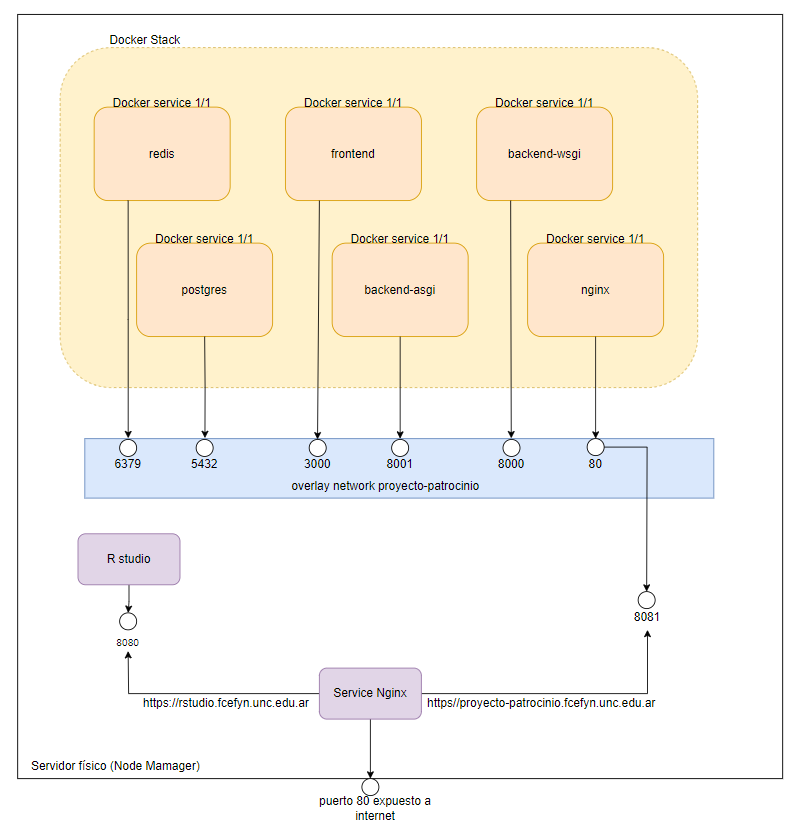
\includegraphics[width=1\linewidth]{fig/deploy.png}
\caption{Diagrama de Despliegue}
\label{fig:deploy-in-server}
\end{figure}

\section{Configuración}

Una vez que la plataforma esté en funcionamiento, el administrador debe acceder al panel web utilizando las credenciales proporcionadas en el archivo de configuración. A continuación, se describen los pasos para realizar la configuración inicial:

\begin{enumerate}
    \item Inicie sesión en la plataforma como administrador.
    \item Ingrese a la siguiente URL: \url{http://{{dominio}}/admin}.
    
    \item Verifique la configuración del dominio en la sección de sitios (Figura \ref{fig:config-sites}). Es esencial asegurarse de que el dominio esté correctamente establecido. Si es necesario realizar cambios, es \textbf{importante}\textbf{ no crear nuevos sitios ni eliminar} el existente, sino editar la información del sitio existente.
\end{enumerate}

\begin{figure}[H]
    \centering
    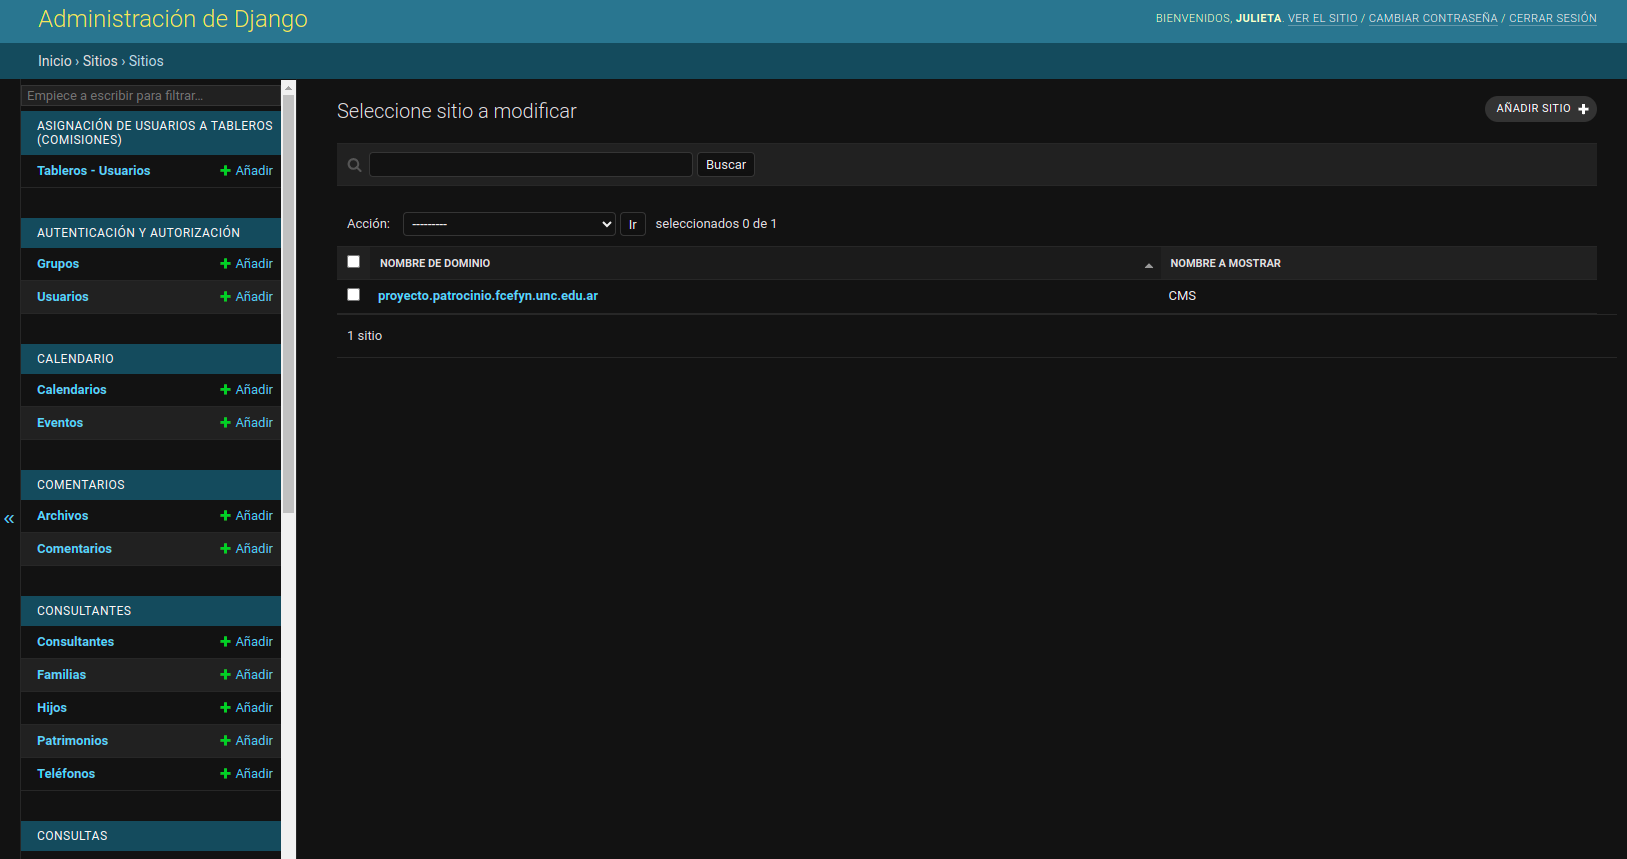
\includegraphics[width=1\linewidth]{fig/sites.png}
    \caption{Configuración de Sitios en el Panel de Administración.}
    \label{fig:config-sites}
\end{figure}


A continuación, el administrador debe crear todas los tableros de trabajo para cada comisión existente en el patrocinio a través de la sección de \textit{Boards} (ver Figura \ref{fig:boards-admin}).

\begin{figure}[H]
    \centering
    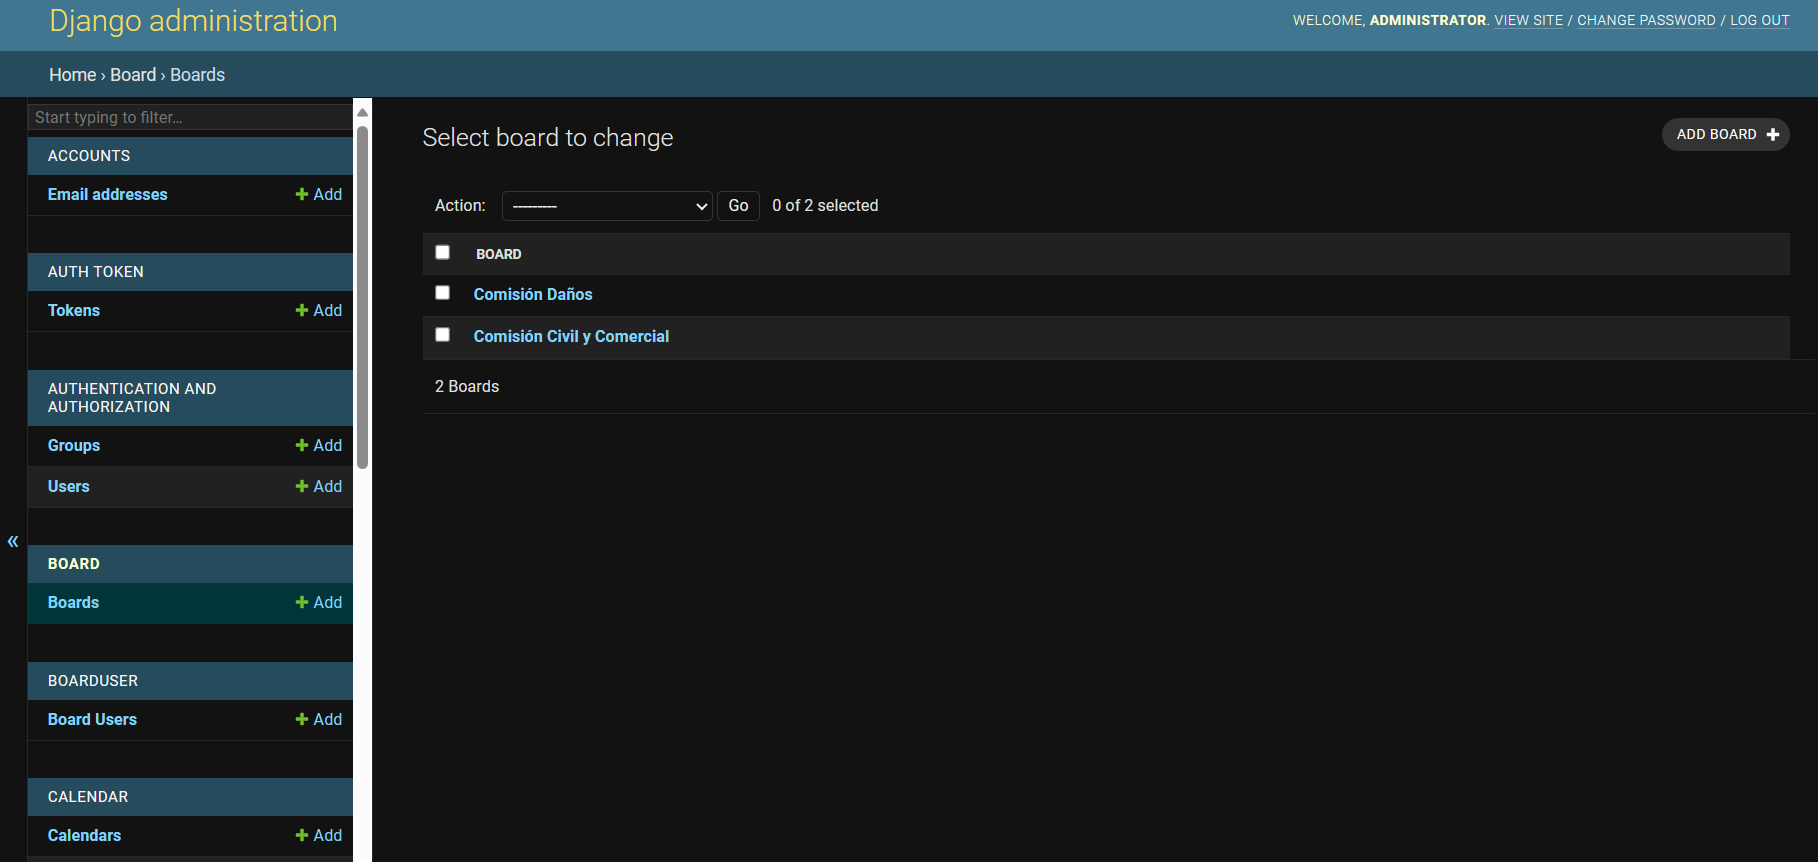
\includegraphics[width=1\linewidth]{fig/boards-admin.png}
    \caption{Creación de Pizarras en la Sección de Administración.}
    \label{fig:boards-admin}
\end{figure}

Finalmente, se deberá registrar una cuenta de usuario para la integración con Google Forms y otorgarle permisos de ``forms''. Para obtener información detallada sobre cómo realizar estos pasos, consulte la sección \ref{sec:registrar-cuenta} para la creación de la cuenta y la sección \ref{subsec:integracion-google-form} para la integración de la cuenta con Google Forms.



\section{Registro de Usuarios}\label{sec:registrar-cuenta}

Para poder registrar un usuario, El usuario deberá seguir los siguientes pasos:

\begin{enumerate}
    \item Ingresar a la página web y seleccionar la opción ``¿No tienes una cuenta? Regístrate'.
    \item Completar los datos requeridos, acepte los términos y condiciones, y haga clic en el botón ``Registrarse'', como se muestra en la Figura \ref{fig:signup}.


    \begin{figure}[H]
        \centering
        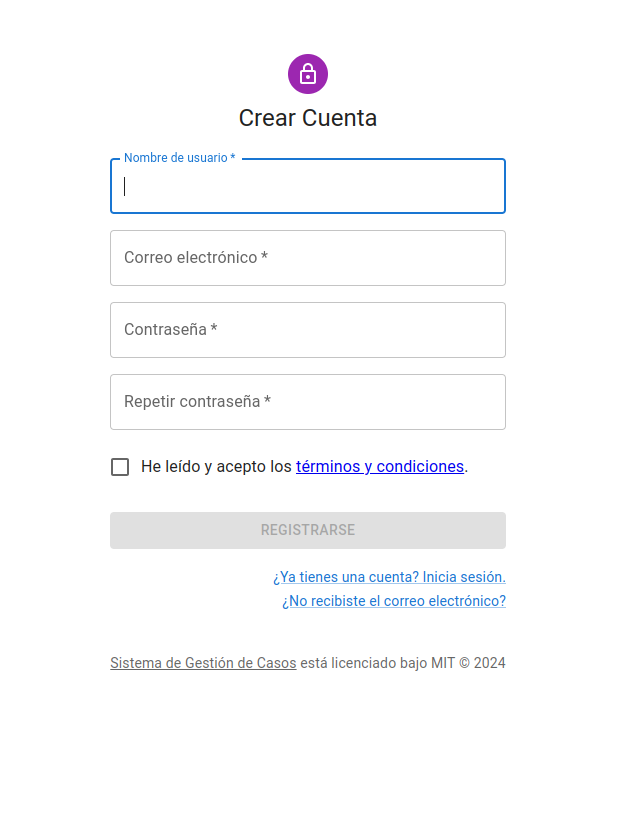
\includegraphics[width=0.7\linewidth]{fig/signup.png}
        \caption{Pantalla de Registro de Usuarios.}
        \label{fig:signup}
    \end{figure}

    \item Revisar la casilla de correlo electrónico y seleccionar el enlace en el correo enviado (ver Figura \ref{fig:confirm-email}).

    \textbf{Nota}: El formato de este email, fue previamente configurado con los templates en la etapa de configuración de software.

    \begin{figure}[H]
        \centering
        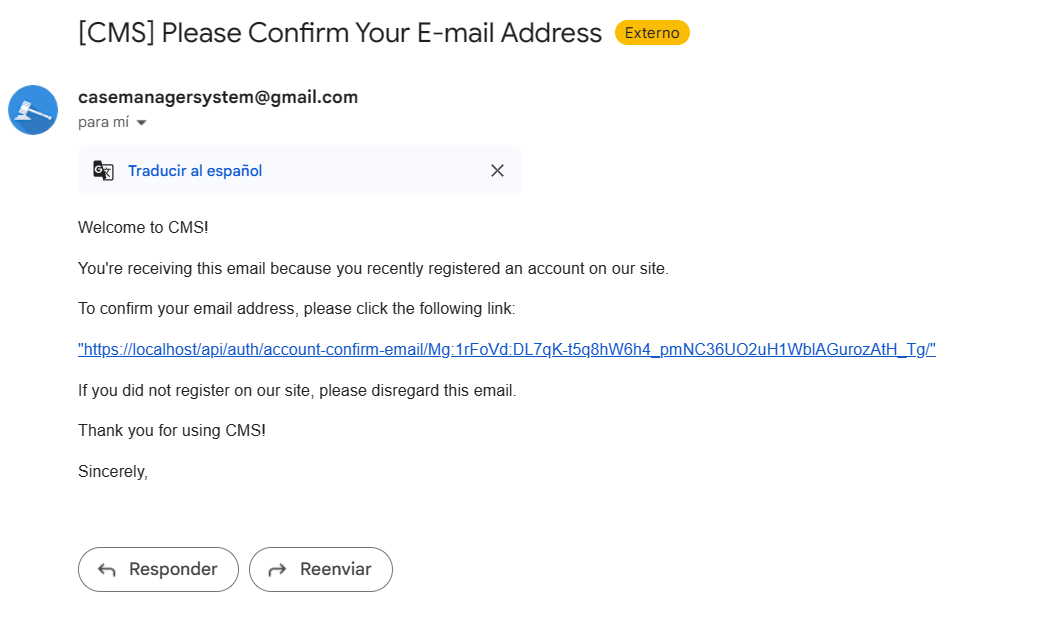
\includegraphics[width=1\linewidth]{fig/confirm-email.png}
        \caption{Confirmación por Correo Electrónico.}
        \label{fig:confirm-email}
    \end{figure}
\end{enumerate}
La página lo redirigirá a la principal, pero aún el usuario no podrá acceder hasta que un administrador habilite su cuenta. Para activar la cuenta, el administrador debe seguir estos pasos:

\begin{enumerate}
    \item Ingresar a la sección de administración y dirigirse a la pestaña de usuarios.
    \item Seleccionar el nuevo usuario y editar la sección de permisos, como se muestra en la figura \ref{fig:user-permission}.


    \begin{figure}[H]
        \centering
        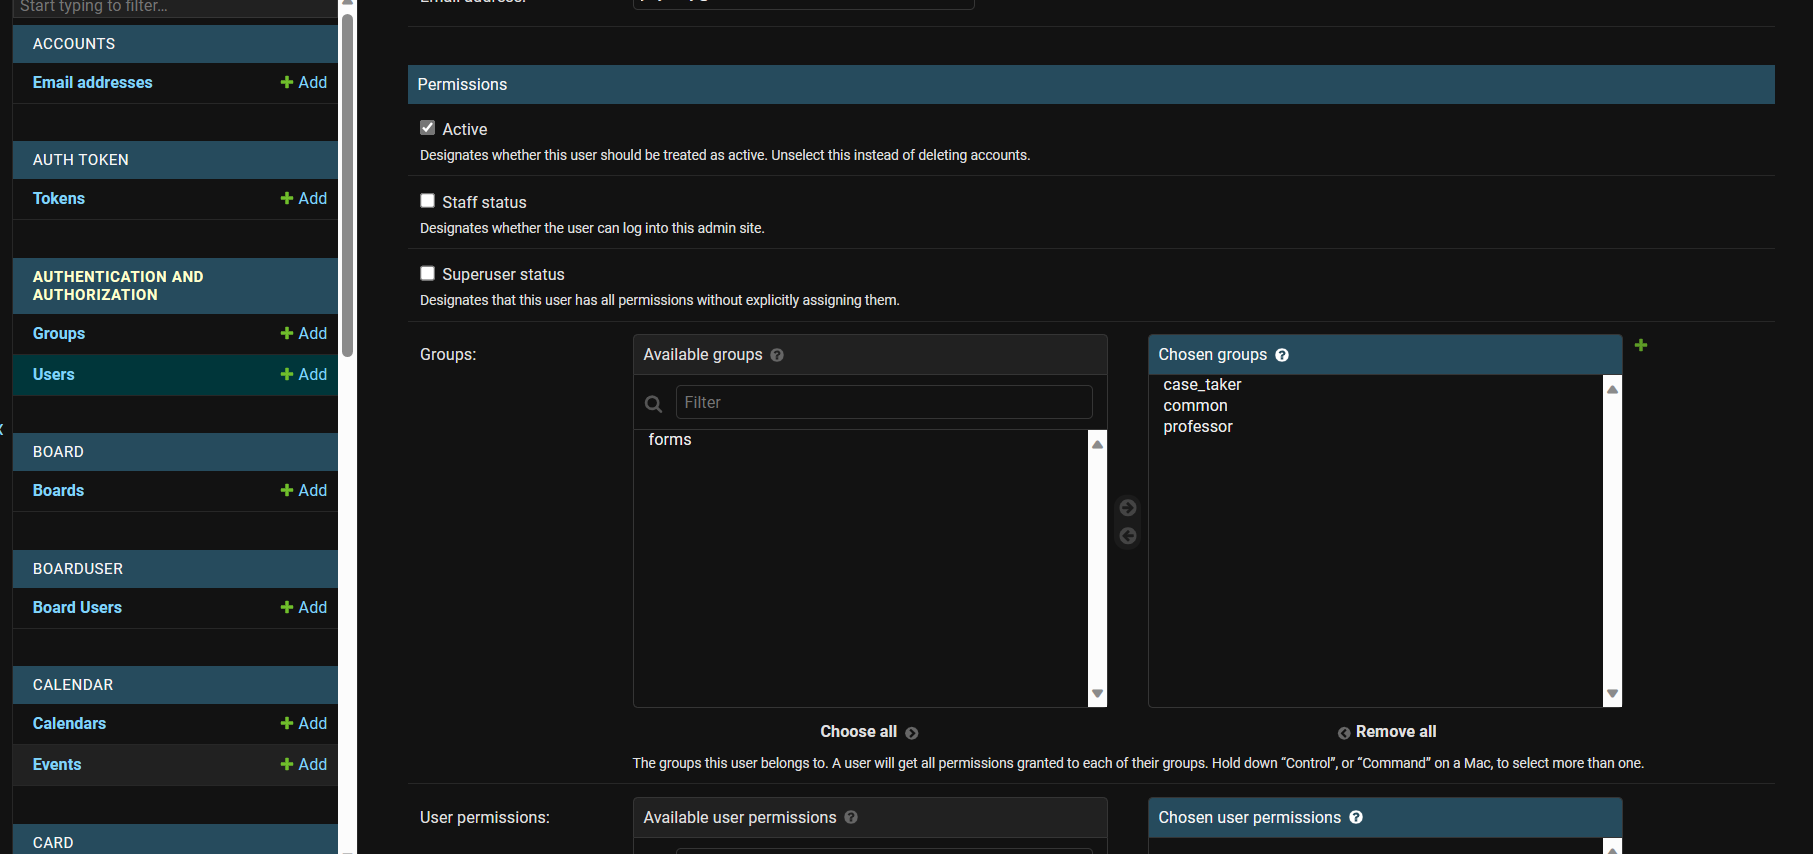
\includegraphics[width=1\linewidth]{fig/user-permission.png}
        \caption{Configuración de Permisos de Usuario.}
        \label{fig:user-permission}
    \end{figure}
    
    \item En la sección, marcar la opción ``Activo'' y otorgar los permisos necesarios (ver \ref{sec:permisos-usuarios}) antes de guardar.

\end{enumerate}

Si el usuario es un miembro de una comisión, el administrador también deberá realizar los siguientes pasos adicionales.

\begin{enumerate}
    \item Ingresar a la sección ``Tableros - Usuarios''.
    \item Crear la relación del usuario con la comisión correspondiente, como se observa en la figura \ref{fig:board-user-2}.

    \begin{figure}[H]
        \centering
        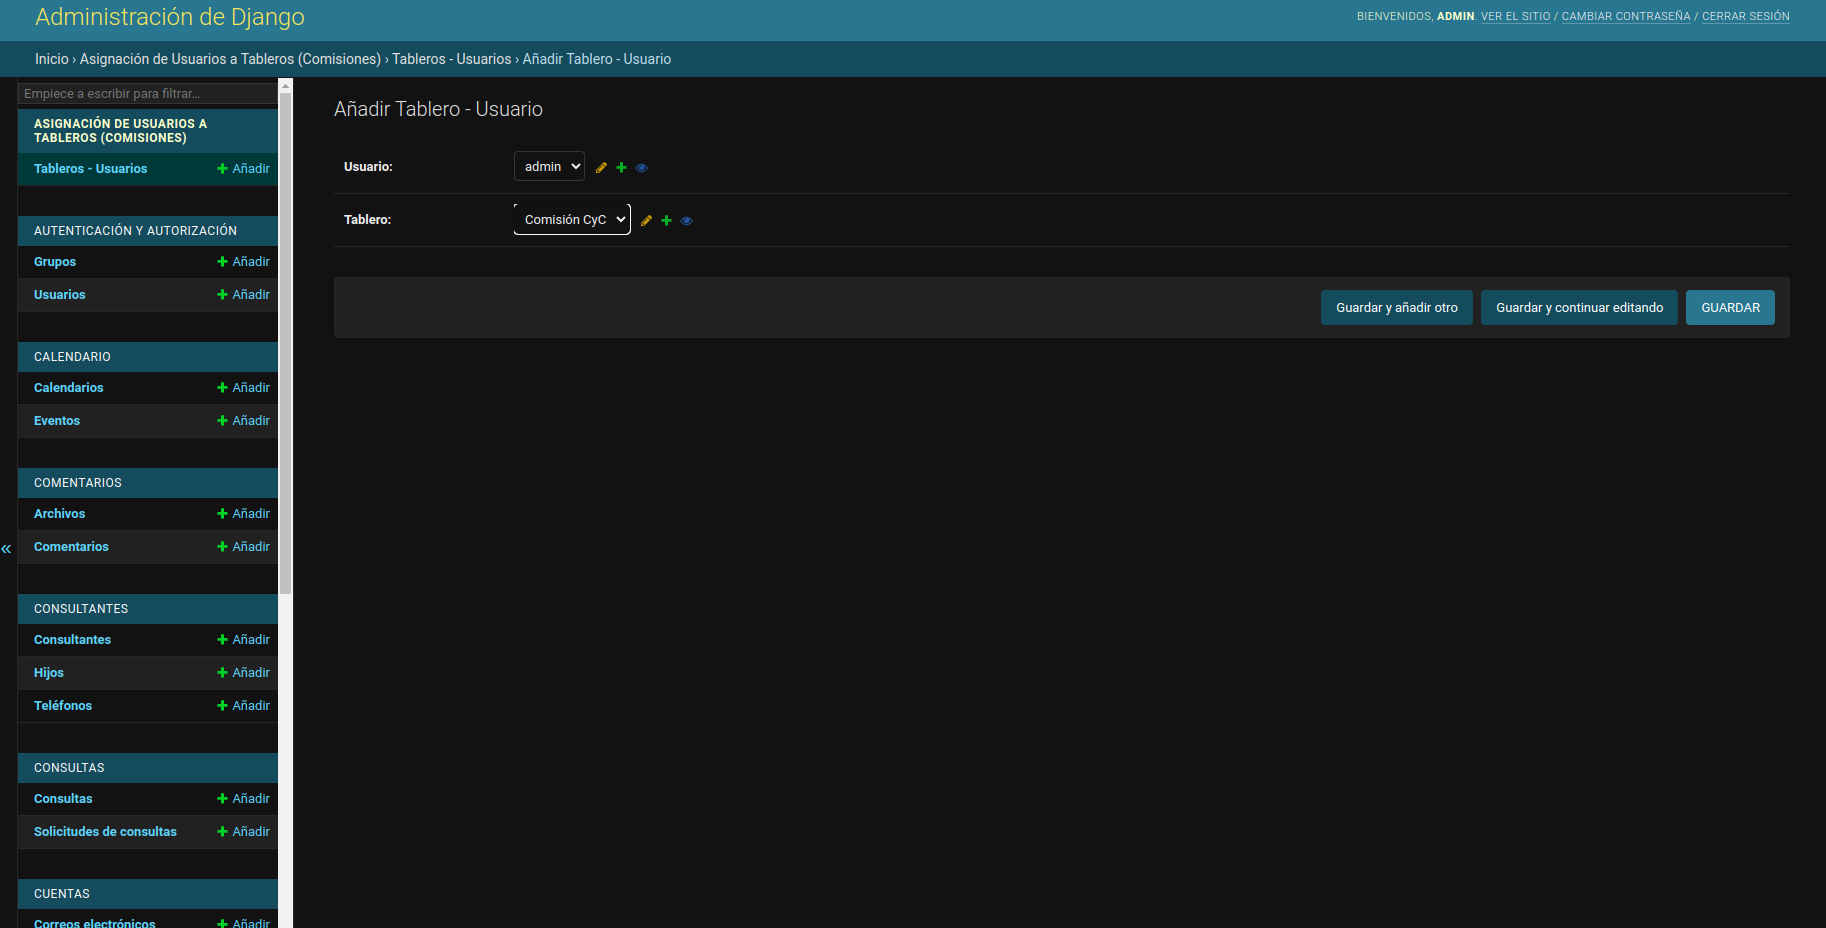
\includegraphics[width=1\linewidth]{fig/board-user.png}
        \caption{Creación de Relación Usuario-Comisión.}
        \label{fig:board-user-1}
    \end{figure}
    
    \begin{figure}[H]
        \centering
        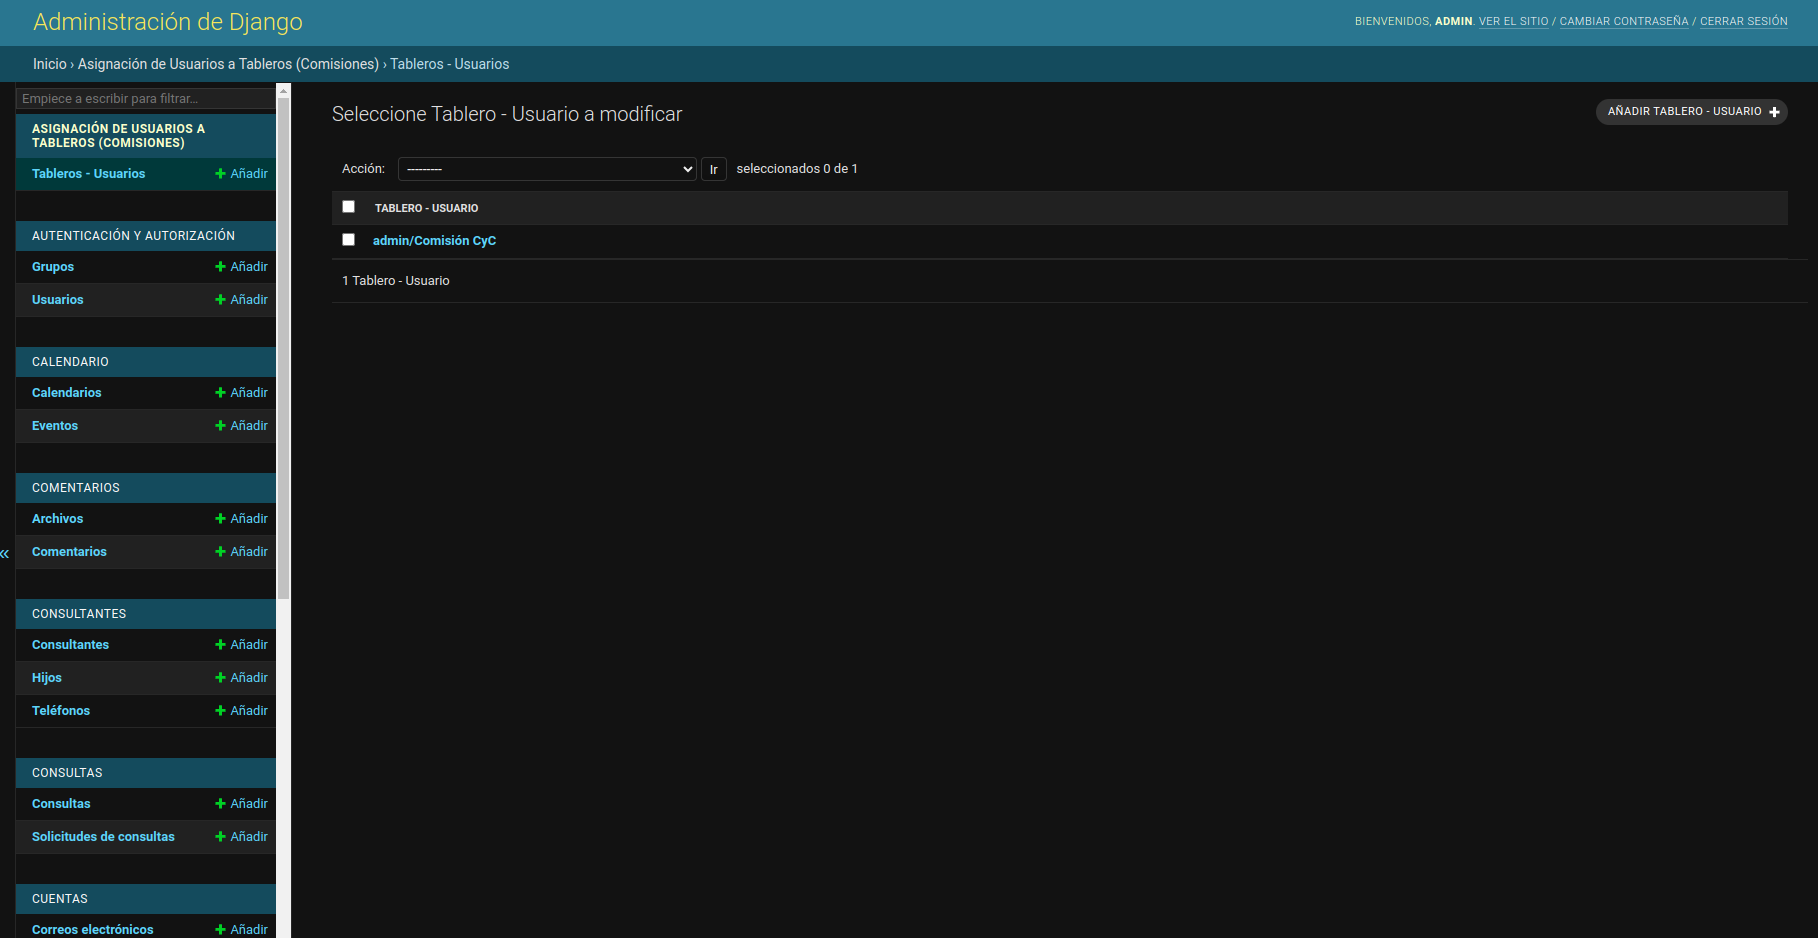
\includegraphics[width=1\linewidth]{fig/board-user-2.png}
        \caption{Lista de Relaciones Usuario-Comisión.}
        \label{fig:board-user-2}
    \end{figure}
\end{enumerate}

Después de completar estos pasos, el usuario podrá iniciar sesión correctamente en la web desde la página de inicio de sesión. La Figura \ref{fig:signin-real-page-2} muestra la página de inicio de sesión.

\begin{figure}[H]
    \centering
    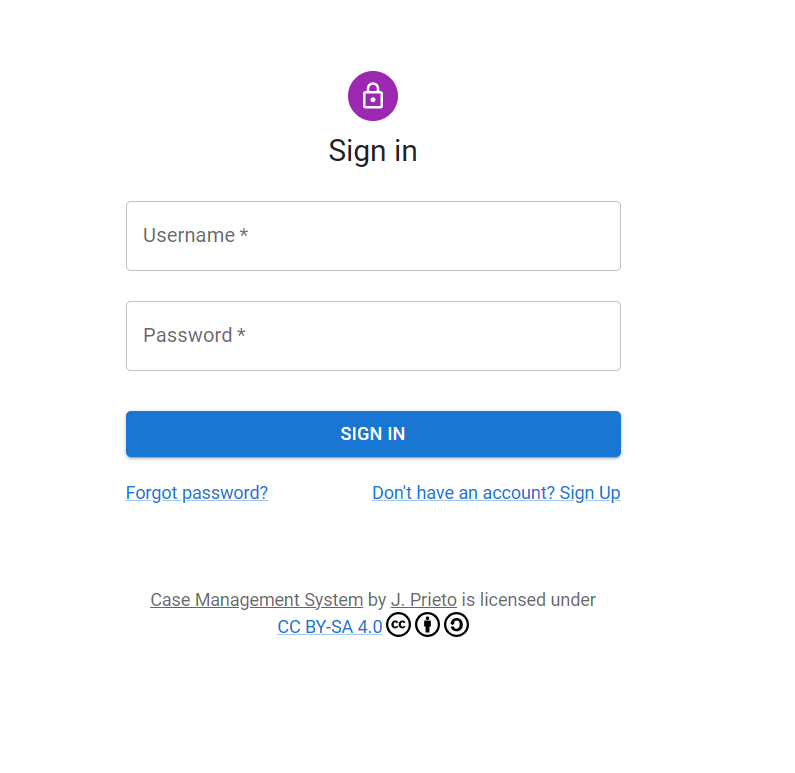
\includegraphics[width=0.7\linewidth]{fig/signin-real-page.png}
    \caption{Página de Inicio de Sesión.}
    \label{fig:signin-real-page-2}
\end{figure}



\section{Permisos de Usuario}\label{sec:permisos-usuarios}

Los grupos de permisos de usuarios se encuentran en la sección "Groupos" de la página de administración y se detallan a continuación:

\begin{table}[H]
    \centering
    \begin{tabular}{|c|p{10cm}|}
        \hline
        \textbf{Grupo} & \textbf{Descripción}\\
        \hline
        common & Grupo de permisos básicos necesarios tanto para un tomador de caso como para un profesor.\\
        \hline
        case\_taker & Grupo de permisos para un tomador de caso. Necesarios para el manejo de la consultoría.\\
        \hline
        professor & Grupo de permisos para un profesor. Necesarios para el manejo de una comisión.\\
        \hline
        forms & Grupo de permisos exclusivo para la cuenta de Google Forms, que le permite registrar formularios.\\
        \hline
    \end{tabular}
    \caption{Grupos de Permisos de Usuario.}
    \label{tab:grupos-permisos-usuario}
\end{table}

\section{Permisos de Usuario}\label{sec:permisos-usuarios}

Los grupos de permisos de usuarios se encuentran en la sección "Groups" de la página de administración y se detallan a continuación:

\begin{table}[H]
    \centering
    \begin{tabular}{|c|p{10cm}|}
        \hline
        \textbf{Grupo} & \textbf{Descripción}\\
        \hline
        common & Grupo de permisos básicos necesarios tanto para un tomador de caso como para un profesor.\\
        \hline
        case\_taker & Grupo de permisos para un tomador de caso. Necesarios para el manejo de la consultoría.\\
        \hline
        professor & Grupo de permisos para un profesor. Necesarios para el manejo de una comisión.\\
        \hline
        forms & Grupo de permisos exclusivo para la cuenta de Google Forms, que le permite registrar formularios.\\
        \hline
    \end{tabular}
    \caption{Grupos de Permisos de Usuario.}
    \label{tab:grupos-permisos-usuario}
\end{table}

\textbf{Nota:} El grupo de permisos \textit{common} debe asignarse junto con \textit{case\_taker} o \textit{professor}.


\section{Administración}\label{sec:administracion}

La página de administración (ver Figura \ref{fig:admin-interface}) proporciona una interfaz amigable para visualizar y gestionar todos los datos del sistema. Al ingresar a la página principal, se presenta una disposición organizada de los datos agrupados en secciones. Además, a la derecha, se muestra un historial de acciones recientes.

\begin{figure}[H]
    \centering
    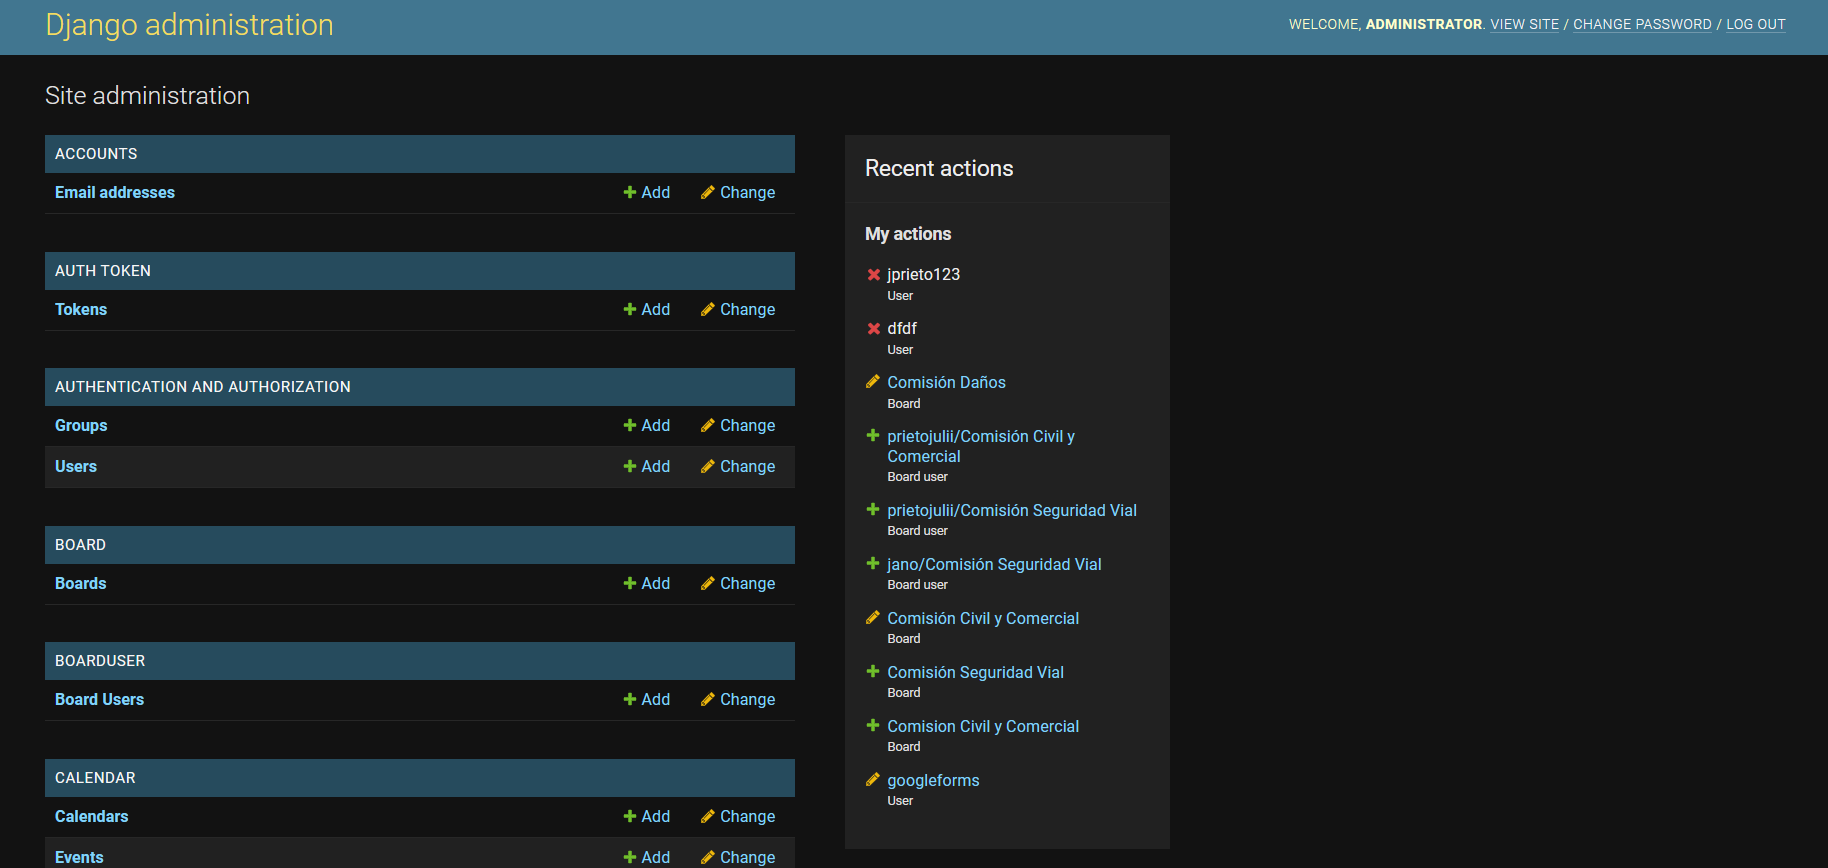
\includegraphics[width=1\linewidth]{fig/administracion.png}
    \caption{Interfaz de Administración de Django.}
    \label{fig:admin-interface}
\end{figure}

En esta interfaz, los administradores pueden realizar diversas acciones, como agregar, editar o eliminar registros, administrar permisos de usuario y conocer el estado del sistma.



\section{Tablero de Trabajo de Consultoría}
La página de consultoría (ver Figura \ref{fig:consultancy-real-page}) es responsable de la administración de las consultas. Aquí, los tomadores de casos pueden revisar las consultas entrantes, representadas como tickets generados a través de formularios de Google. Pueden analizarlas y verificar si cumplen con las condiciones para ser patrocinadas por la entidad. Los tomadores de casos tienen la capacidad de crear, editar y eliminar consultas o enviarlas a una comisión para solicitar patrocinio.

La página está estructurada mediante paneles. El panel izquierdo contiene las consultas sin asignar, mientras que los paneles siguientes representan comisiones, cada uno con los tickets de las solicitudes de asignación. Para asignar una consulta a una comisión, basta con arrastrar la consulta al tablero de la comisión deseada. También es posible eliminar la solicitud volviendo a arrastrar el ticket al panel izquierdo. Para eliminar el ticket, simplemente posicione el mouse sobre el mismo, seleccione el menú que aparecerá y elija la opción ``eliminar``.

\begin{figure}[H]
    \centering
    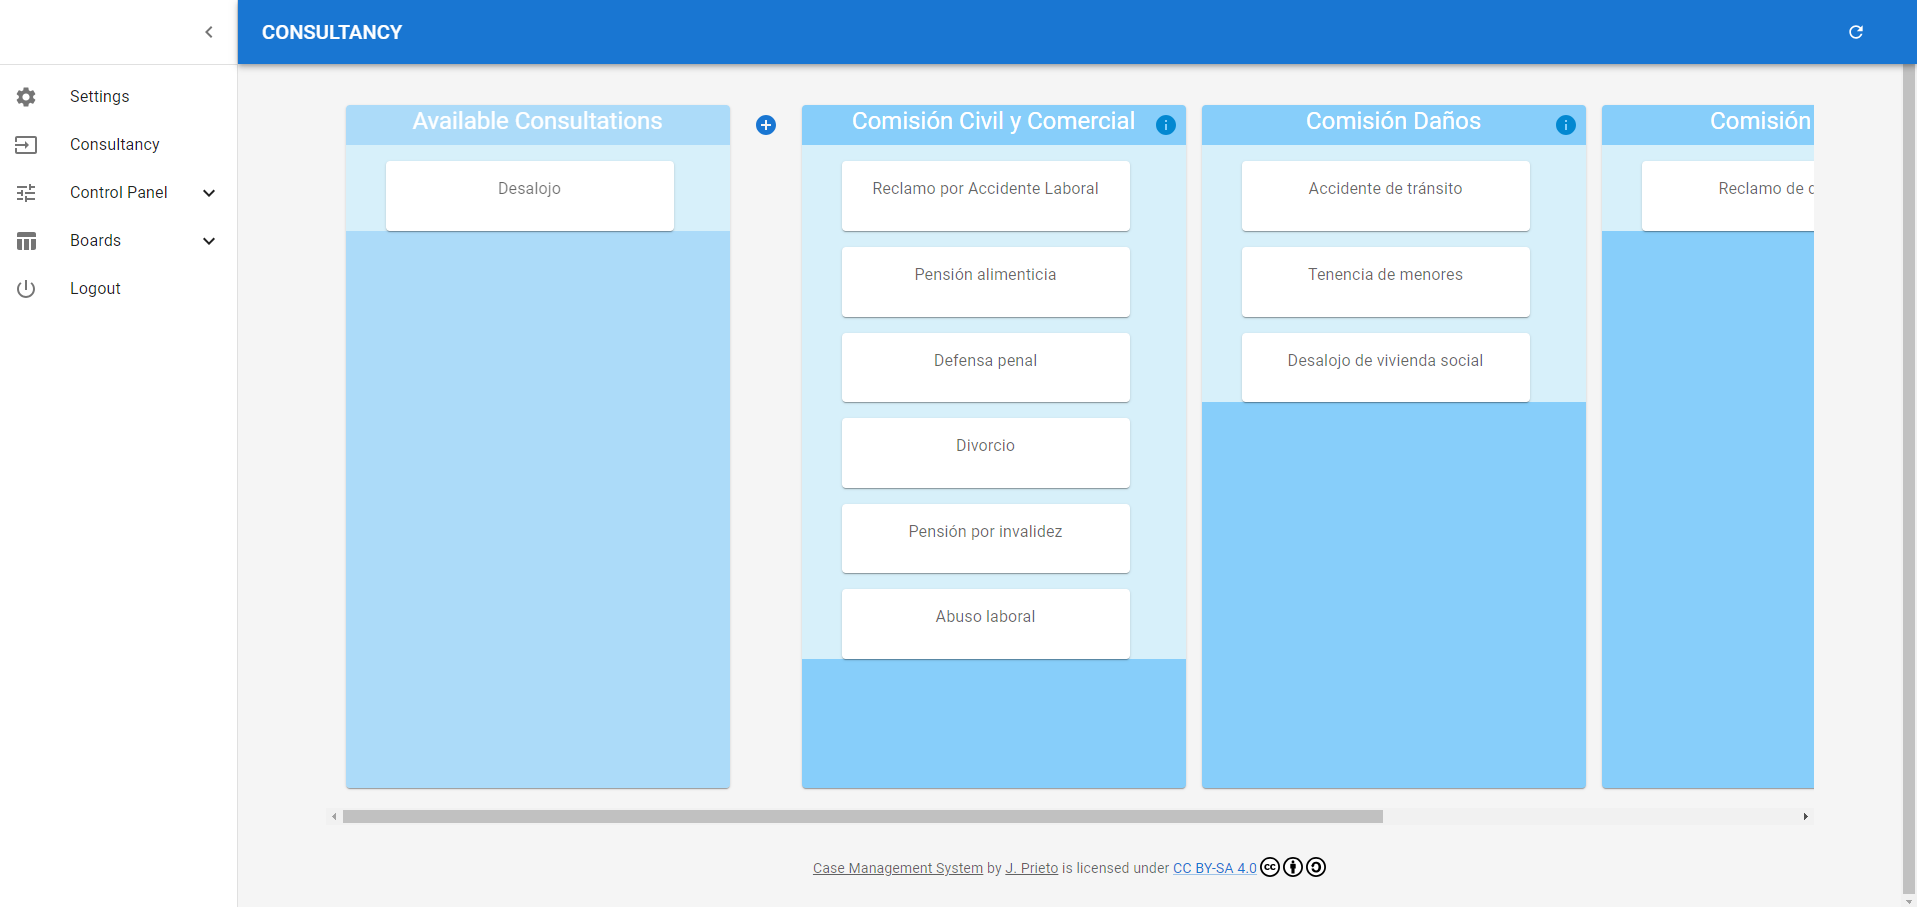
\includegraphics[width=1\linewidth]{fig/consultancy-real-page.png}
    \caption{Página de Consultoría}
    \label{fig:consultancy-real-page}
\end{figure}

Es importante mantener un registro del estado de cada comisión. Cada panel cuenta con un popper en el sector superior derecho que, al hacer clic, muestra la cantidad de consultas asignadas y la cantidad de consultas por estado (por hacer, en progreso o pausadas/bloqueadas). Además, como se ve en la figura \ref{fig:consultancy-logs-1}, incluye un historial de las asignaciones de los últimos 10 días, que muestra la ``etiqueta'' de la consulta y la fecha de asignación.

\begin{figure}[H]
    \centering
    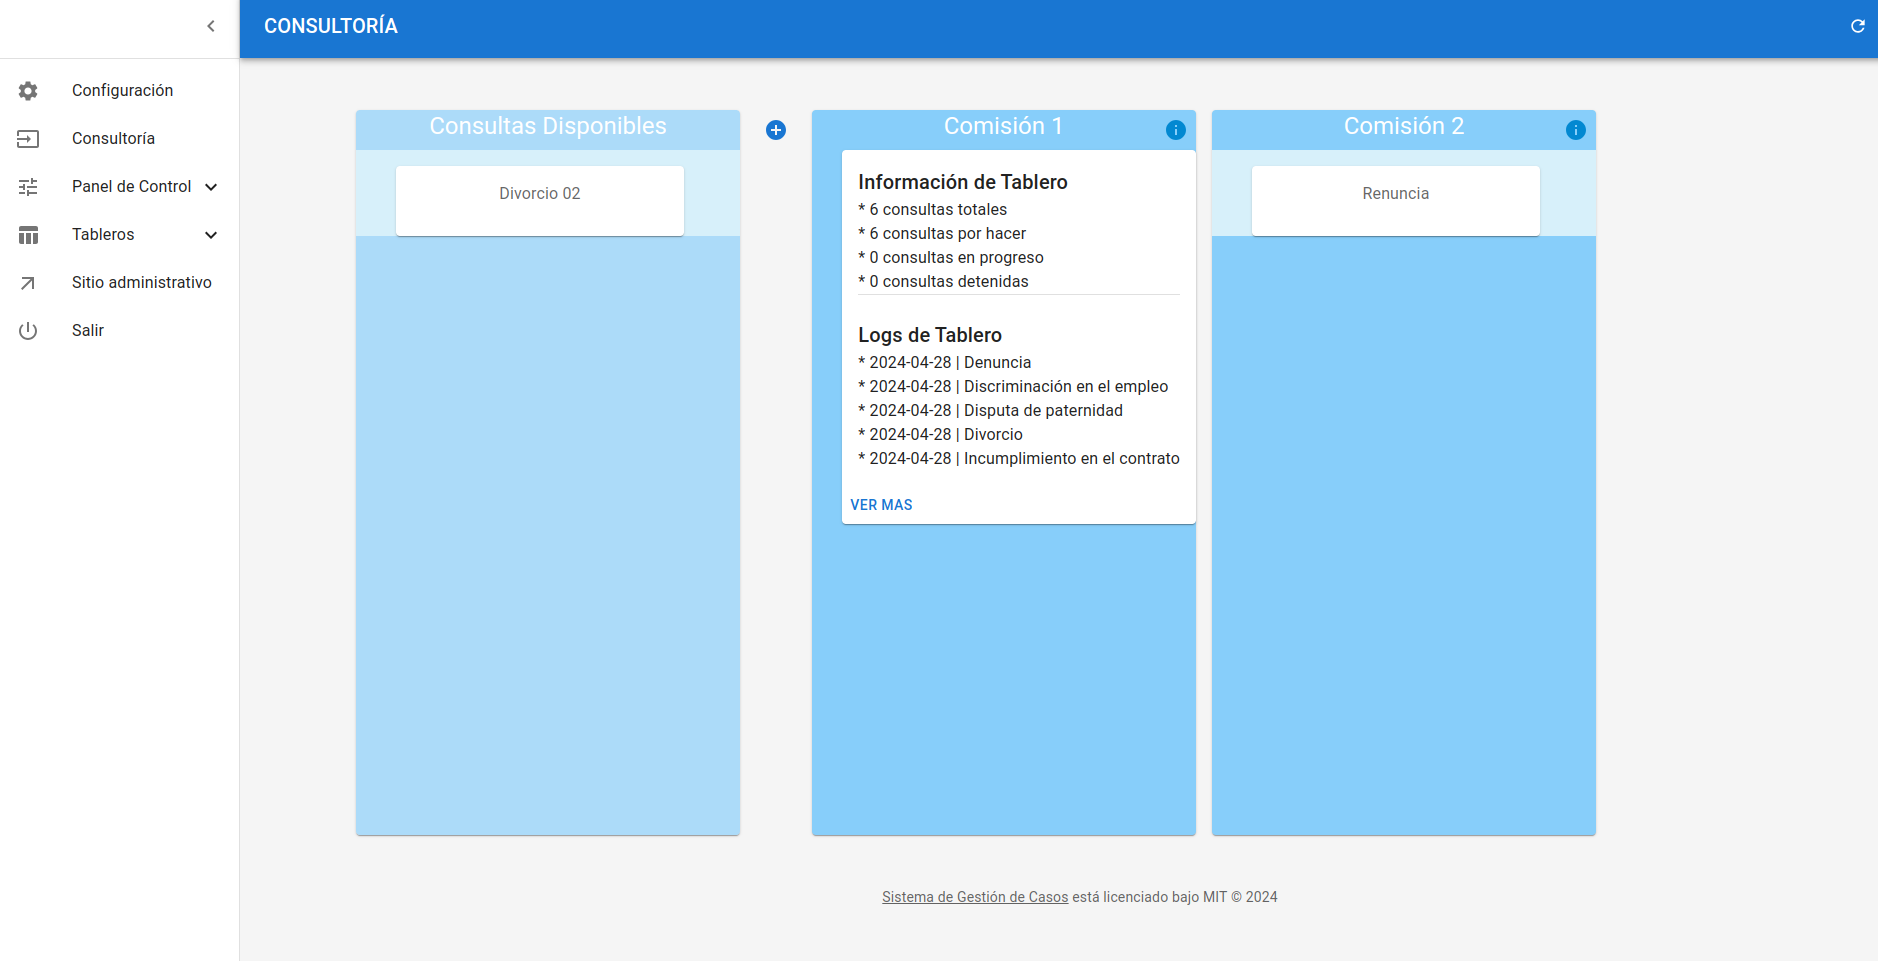
\includegraphics[width=1\linewidth]{fig/consultancy-real-page-logs-1.png}
    \caption{Historial de Asignaciones de una Comisión}
    \label{fig:consultancy-logs-1}
\end{figure}

Cuando la cantidad de consultas asignadas a la comisión en los últimos 10 días es extensa, aparecerá la opción ``ver mas'', que expandirá un panel con todas las asignaciones (ver Figura \ref{fig:consultancy-logs-2}).

\begin{figure}[H]
    \centering
    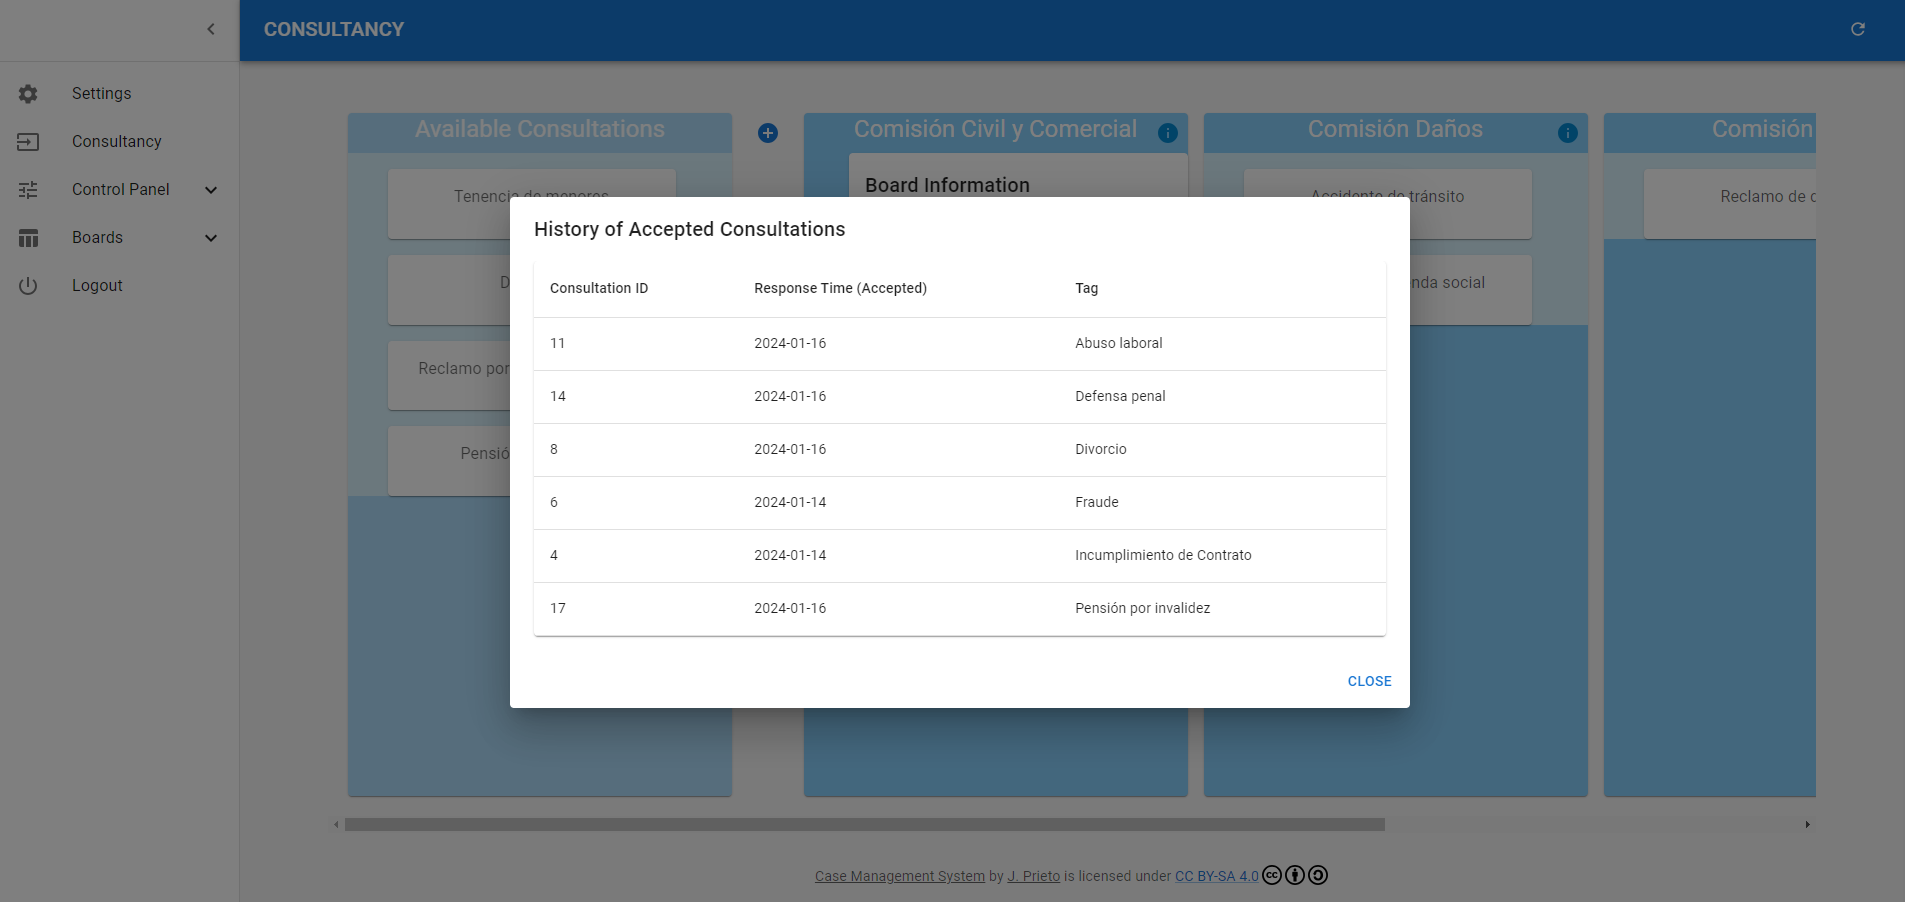
\includegraphics[width=1\linewidth]{fig/consultancy-real-page-logs-2.png}
    \caption{Panel Expandido de Historial de Asignaciones de una Comisión}
    \label{fig:consultancy-logs-2}
\end{figure}

El Usuario Tomador de Caso tiene la capacidad de crear consultas a través de la página de consultoría. Para hacerlo, se selecciona el botón con el símbolo ``+'' ubicado en el panel de entrada, y luego se completa el formulario como se muestra en la figura \ref{fig:formulario-crear-consulta}.

\begin{figure}[H]
    \centering
    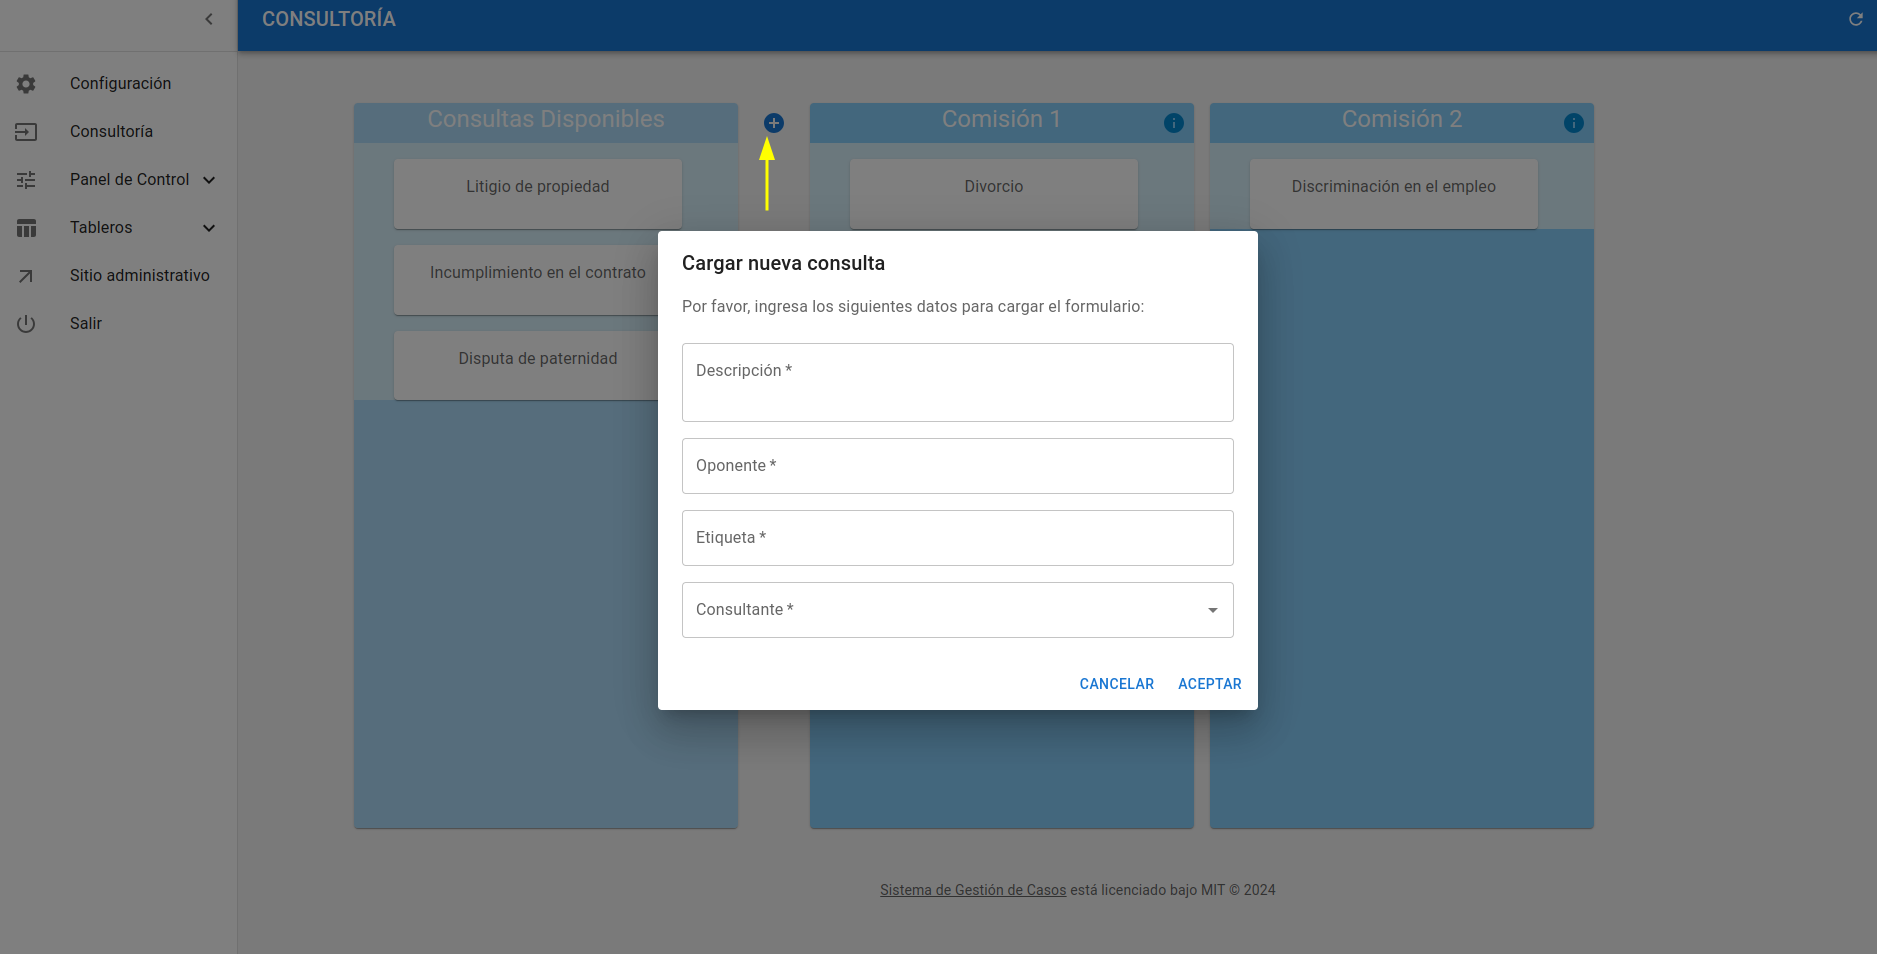
\includegraphics[width=1\linewidth]{fig/crear-consulta-consultancy.png}
    \caption{Formulario para Crear Consulta en la Página de Consultoría}
    \label{fig:formulario-crear-consulta}
\end{figure}




\section{Panel de Control}
El panel de control (ver Figura \ref{fig:consultations-table}) consta de dos pestañas principales: ``Consultas'' y ``Consultantes''. Ambas pestañas ofrecen tablas que pueden descargarse en formato PDF o CSV. Además, proporcionan opciones de filtro y permiten la edición, creación o eliminación de registros.

A continuación, se presenta la pestaña de ``Consultations'', que muestra una tabla con todas las consultas.

\begin{figure}[H]
    \centering
    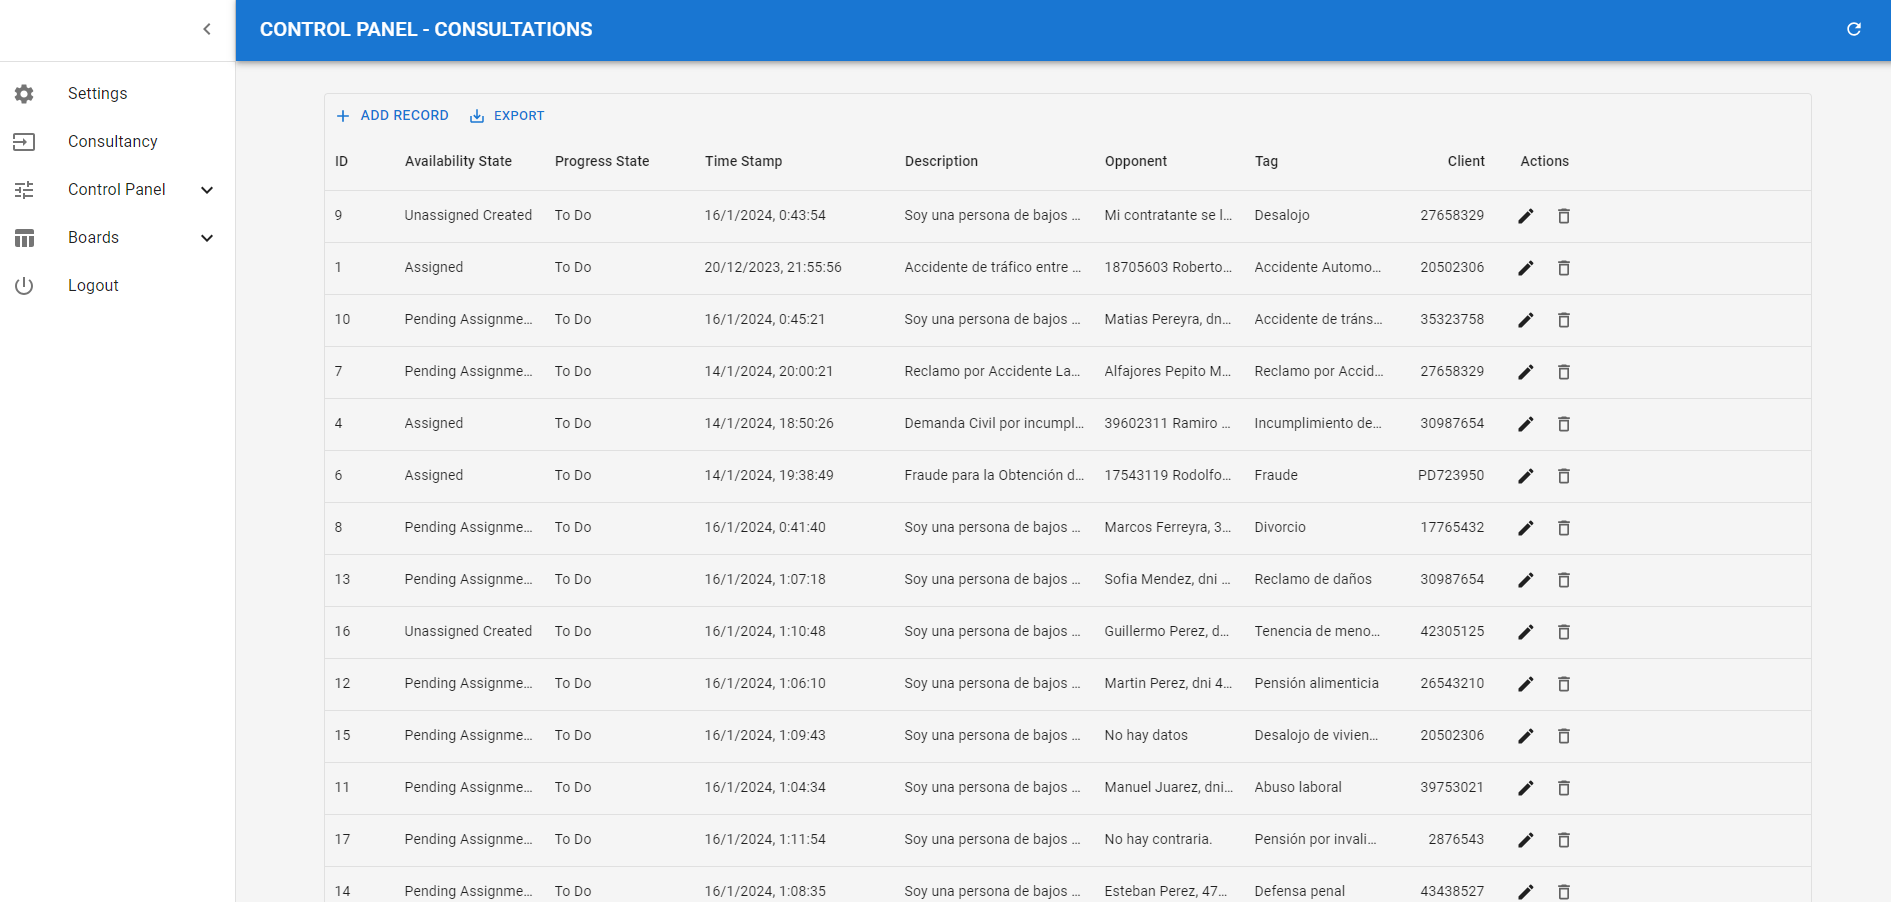
\includegraphics[width=1\linewidth]{fig/consultation-real-page.png}
    \caption{Tabla de Consultas en el Panel de Control.}
    \label{fig:consultations-table}
\end{figure}


En la figura \ref{fig:clients-table}, se presenta la pestaña ``Consultantes'', que muestra una tabla con todos los consultantes.

\begin{figure}[H]
    \centering
    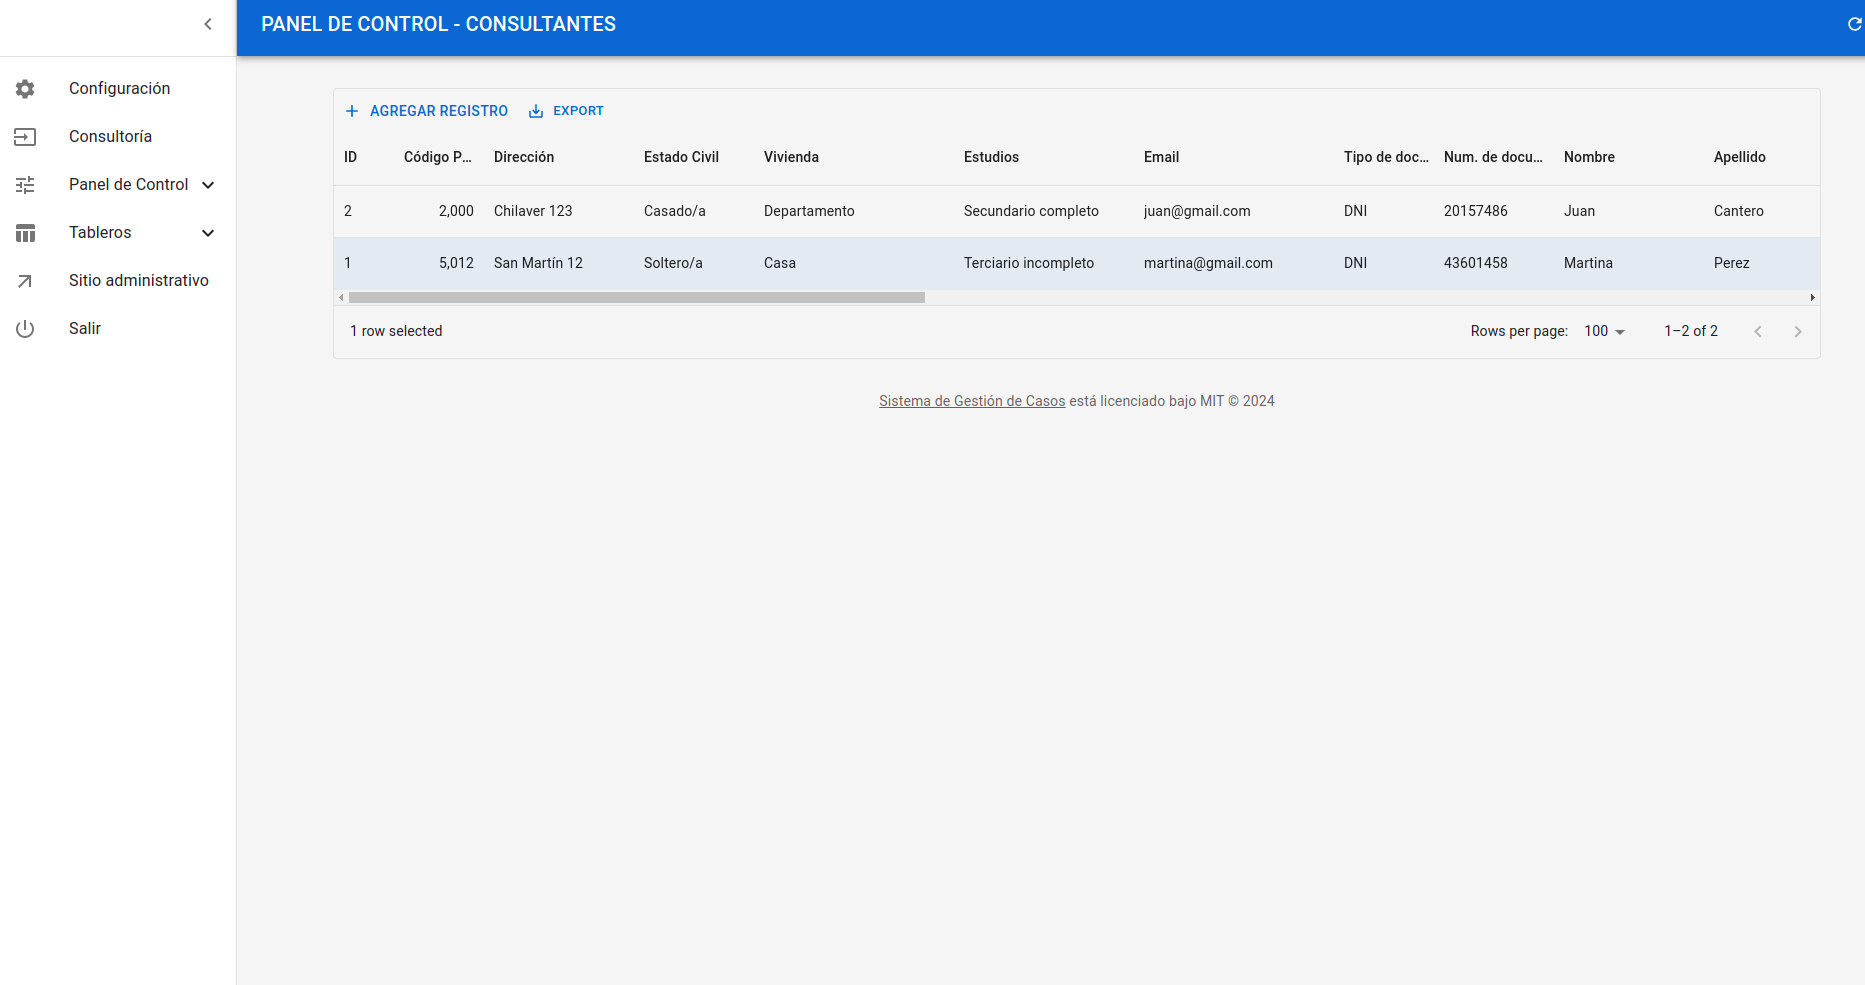
\includegraphics[width=1\linewidth]{fig/clients-real-page.png}
    \caption{Tabla de Clientes en el Panel de Control.}
    \label{fig:clients-table}
\end{figure}

Cada entrada en esta tabla puede ser eliminada o editada seleccionando los elementos en la última columna a la derecha de la entrada deseada. Además, es posible crear un nuevo registro haciendo clic en el botón ``Agregar Registro'' en la parte superior.

La tabla también permite aplicar filtros a algunas de sus columnas (ver Figura \ref{fig:tabla-filtro-ejemplo}). Para ello, cada columna tiene un tooltip que facilita la ordenación ascendente o descendente, filtrado y ocultamiento de la columna. A continuación, se muestra un ejemplo de aplicación de un filtro a la columna ``estado de progreso'' de la tabla ``consultas''.

\begin{figure}[H]
    \centering
    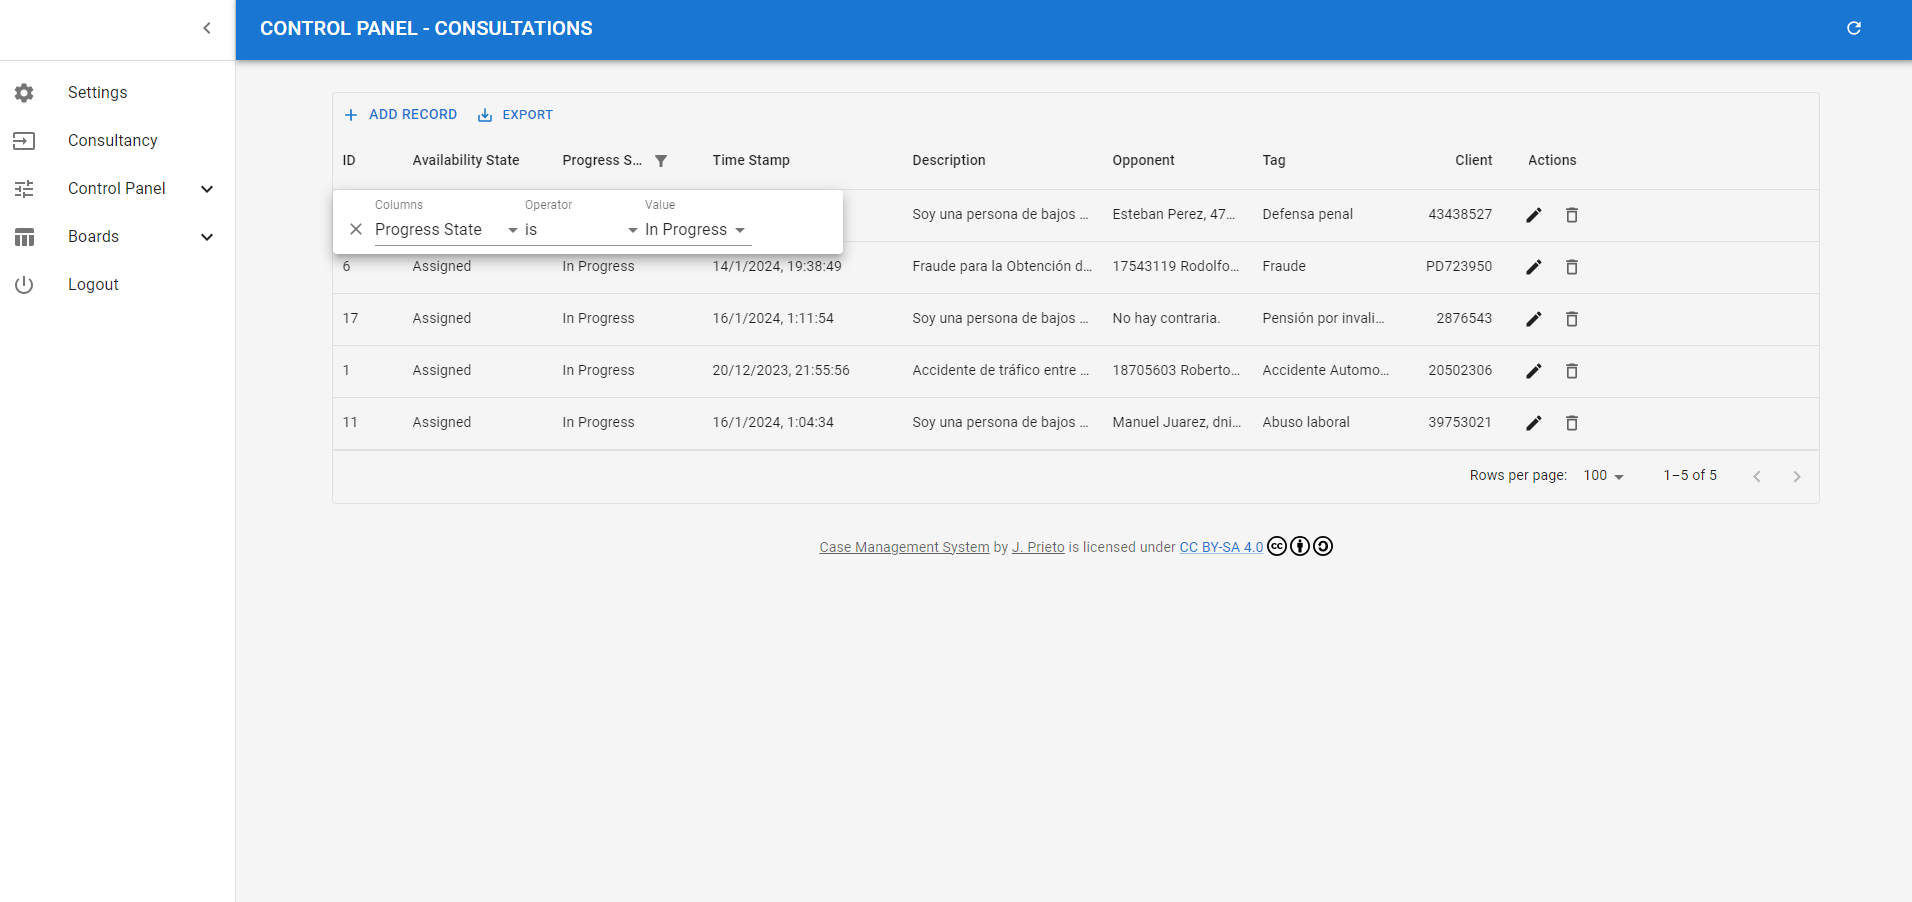
\includegraphics[width=1\linewidth]{fig/tabla-filter.png}
    \caption{Aplicación de un Filtro en la Columna Progress State}
    \label{fig:tabla-filtro-ejemplo}
\end{figure}



\section{Tablero de Trabajo para la Comisión}
Cada comisión cuenta con un ``Tablero'' (ver Figura \ref{fig:board-real-page}), el cual los usuarios con acceso podrán visualizar desde la sección ``Tableros'' en el menú desplegable de la página.

Este espacio está organizado en paneles, siendo el primero a la izquierda el panel de entrada de solicitudes de asignación de casos. Para aceptar una solicitud, basta con arrastrar el ticket de la consulta a alguno de los paneles internos del board. Para rechazarla, se puede seleccionar la opción ``rechazado'' desde el menú del ticket, el cual se hace visible acercando el ratón sobre él.

Los paneles a la izquierda son flexibles y pueden ser creados según la necesidad del usuario, ya sea como organizadores, separadores de consultas, o para cualquier otro agrupamiento conveniente. Por ejemplo, podrían ser utilizados un panel por profesor, otro por estado de progreso de las consultas, o cualquier otro criterio de agrupación preferido.

\begin{figure}[H]
    \centering
    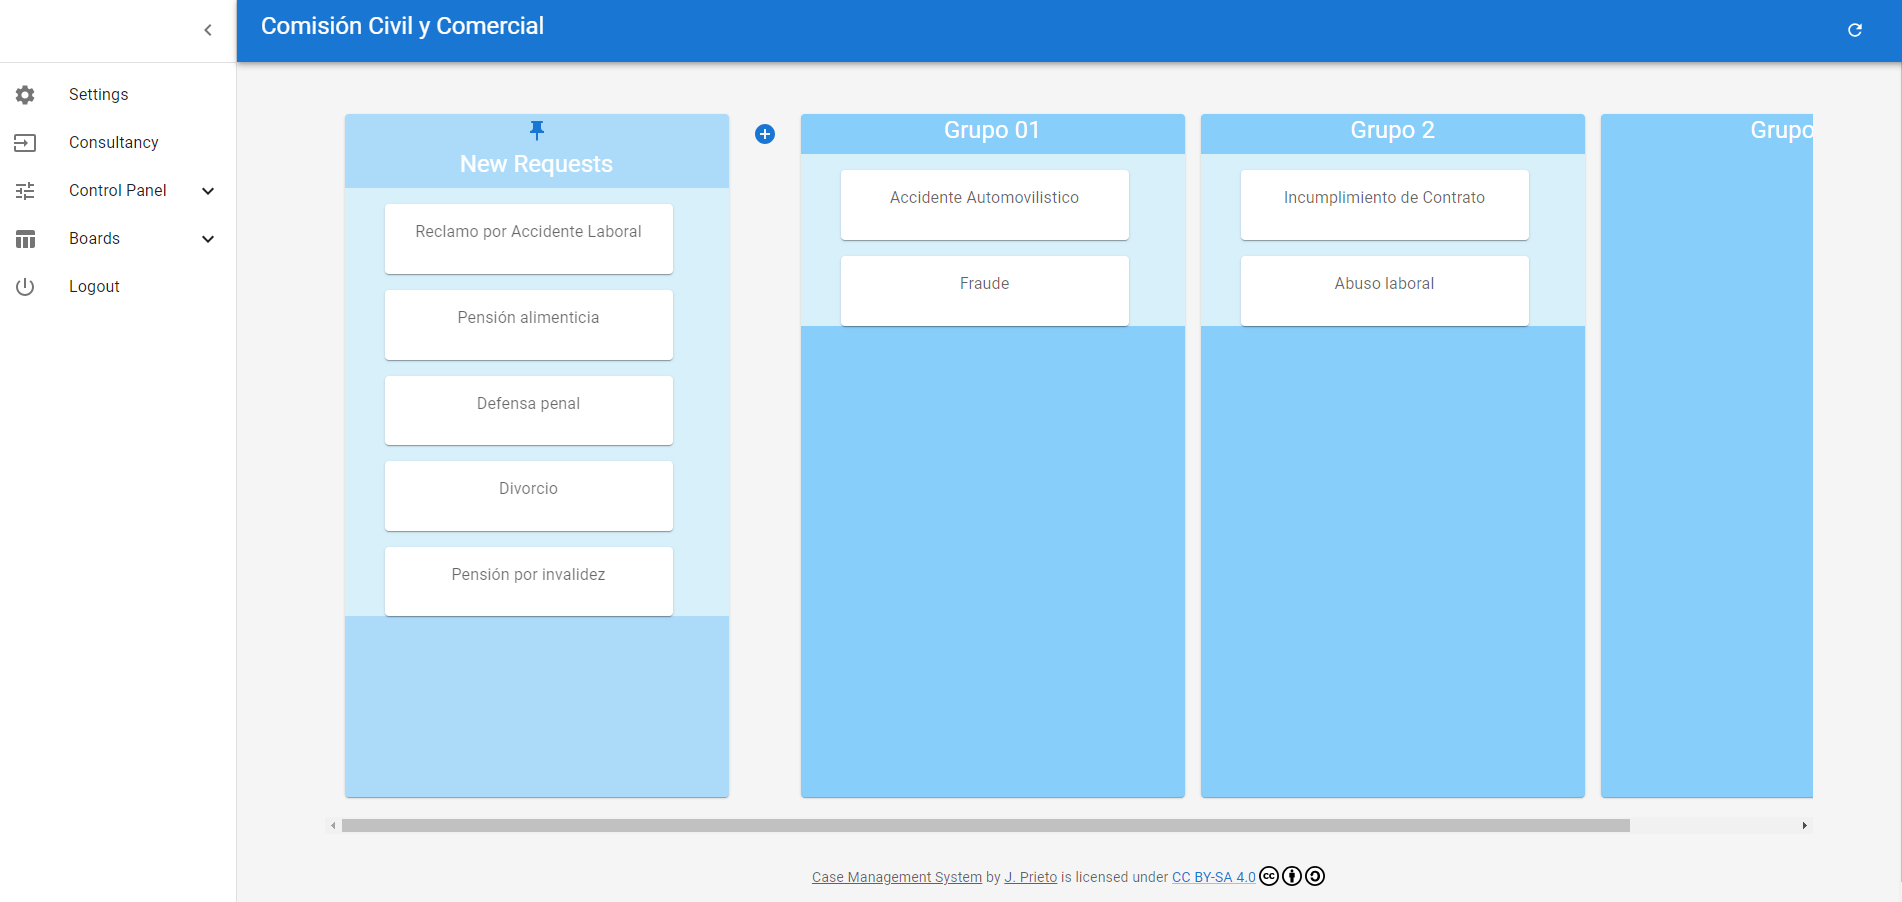
\includegraphics[width=1\linewidth]{fig/board-real-page.png}
    \caption{Página Board de la Comisión}
    \label{fig:board-real-page}
\end{figure}

Cada panel se puede crear utilizando el botón ``+'' e ingresando el nombre correspondiente. Asimismo, se pueden eliminar a través del menú del panel o editar el título haciendo doble clic sobre él (siempre y cuando no existan tickets en el tablero). Además, el board puede ser renombrado haciendo doble clic sobre el título.

La Figura \ref{fig:delete-panel} muestra los botones para eliminar o crear un panel del board.


\begin{figure}[H]
    \centering
    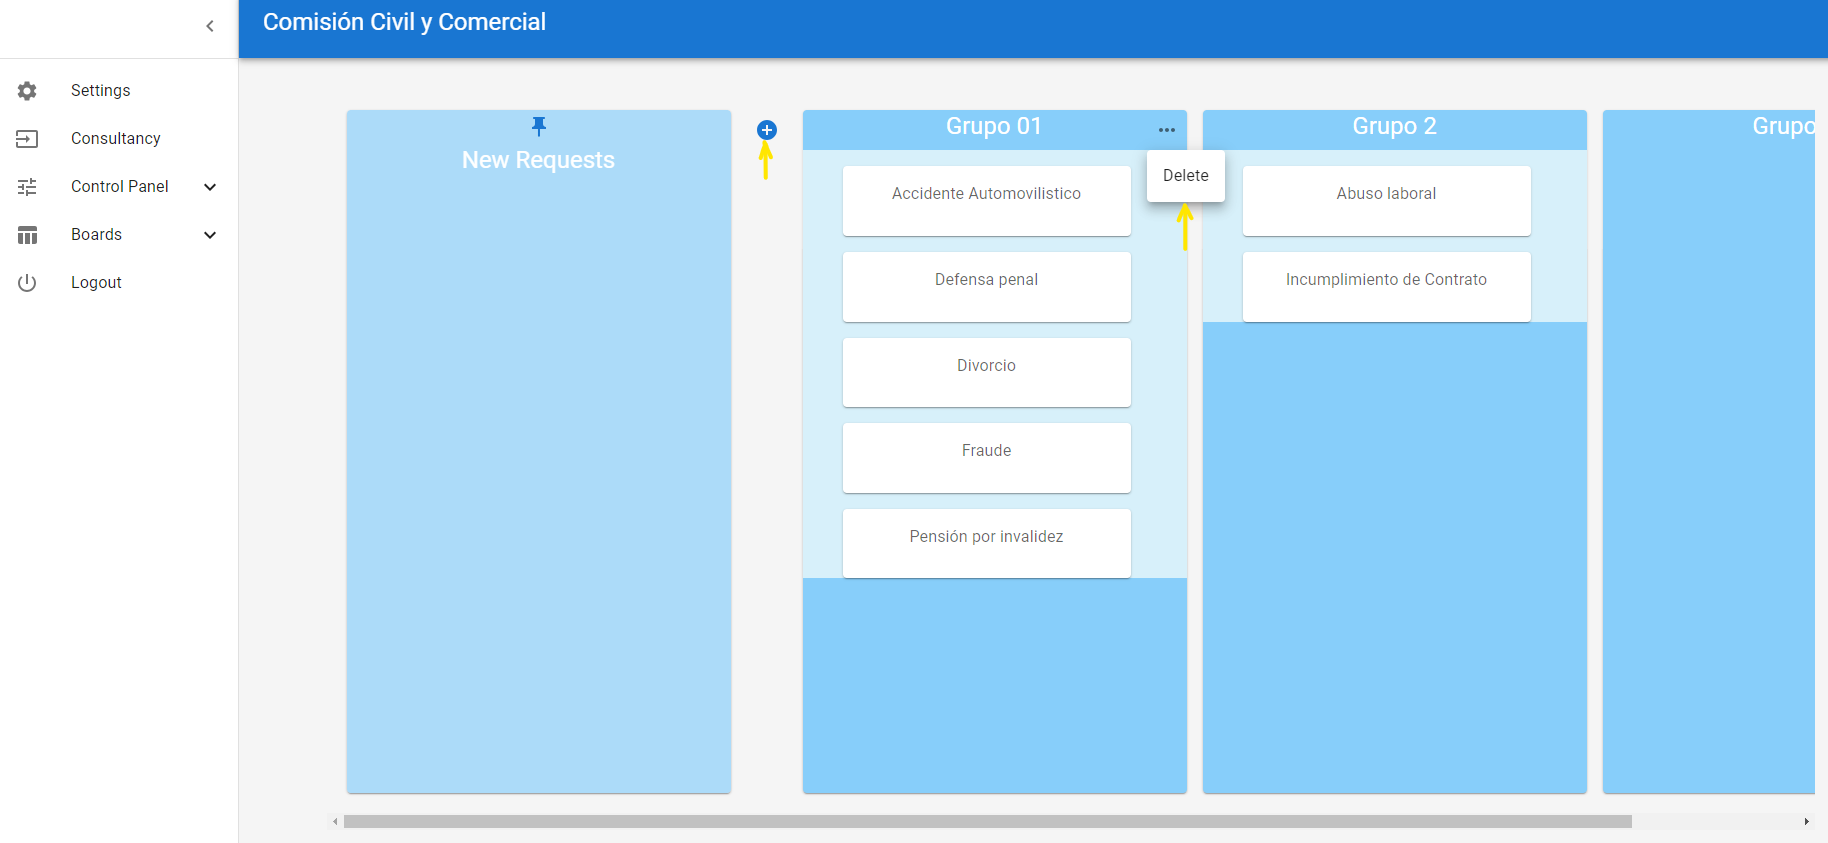
\includegraphics[width=1\linewidth]{fig/delete-panel.png}
    \caption{Botones para eliminar o crear un Panel del Board}
    \label{fig:delete-panel}
\end{figure}





\section{Detalles de la Consulta}\label{sec:info-consulta}

Para obtener más detalles sobre una consulta específica, se debe hacer click en la tarjeta correspondiente, lo que desplegará un cuadro con tres pestañas distintas, como se ve en la figura \ref{fig:consulta-info}.

\begin{figure}[H]
    \centering
    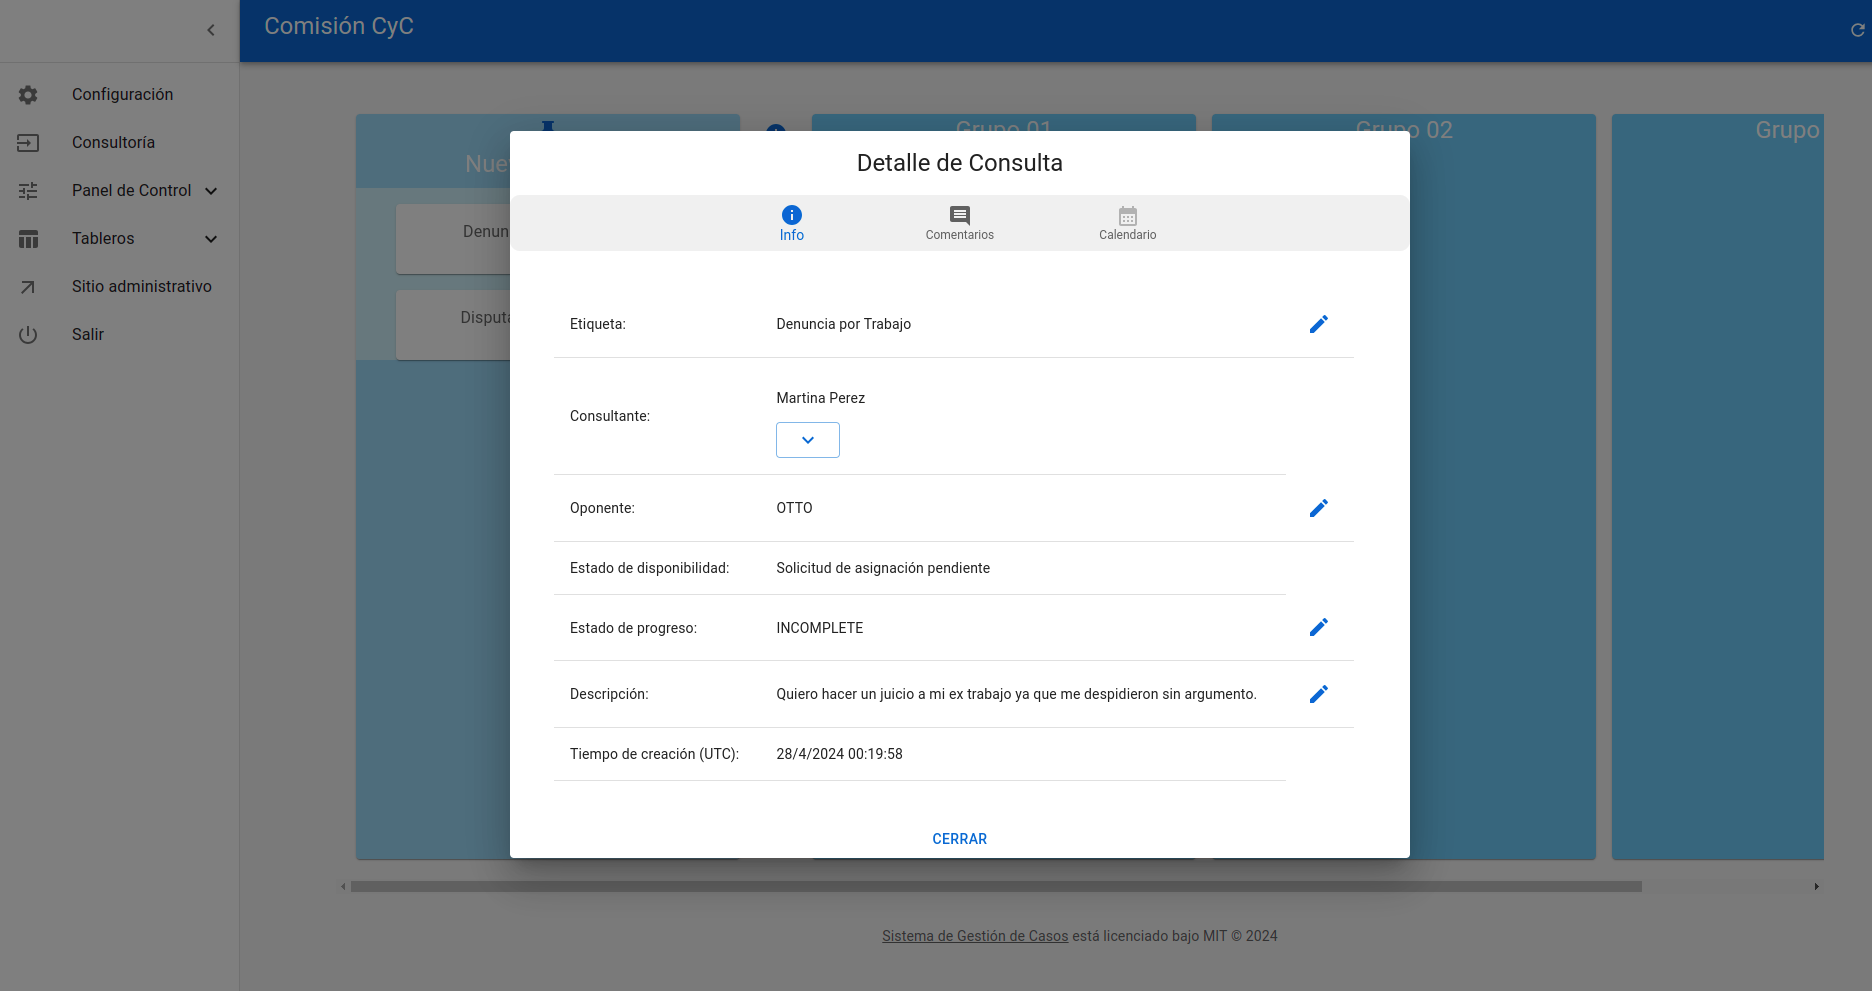
\includegraphics[width=1\linewidth]{fig/info-consulta.png}
    \caption{Ventana de Información de Consulta.}
    \label{fig:consulta-info}
\end{figure}

En la figura \ref{fig:consulta-comentarios}, muestra la primera pestaña, la cual presenta información organizada sobre el consultante y los detalles de la consulta.

\begin{figure}[H]
    \centering
    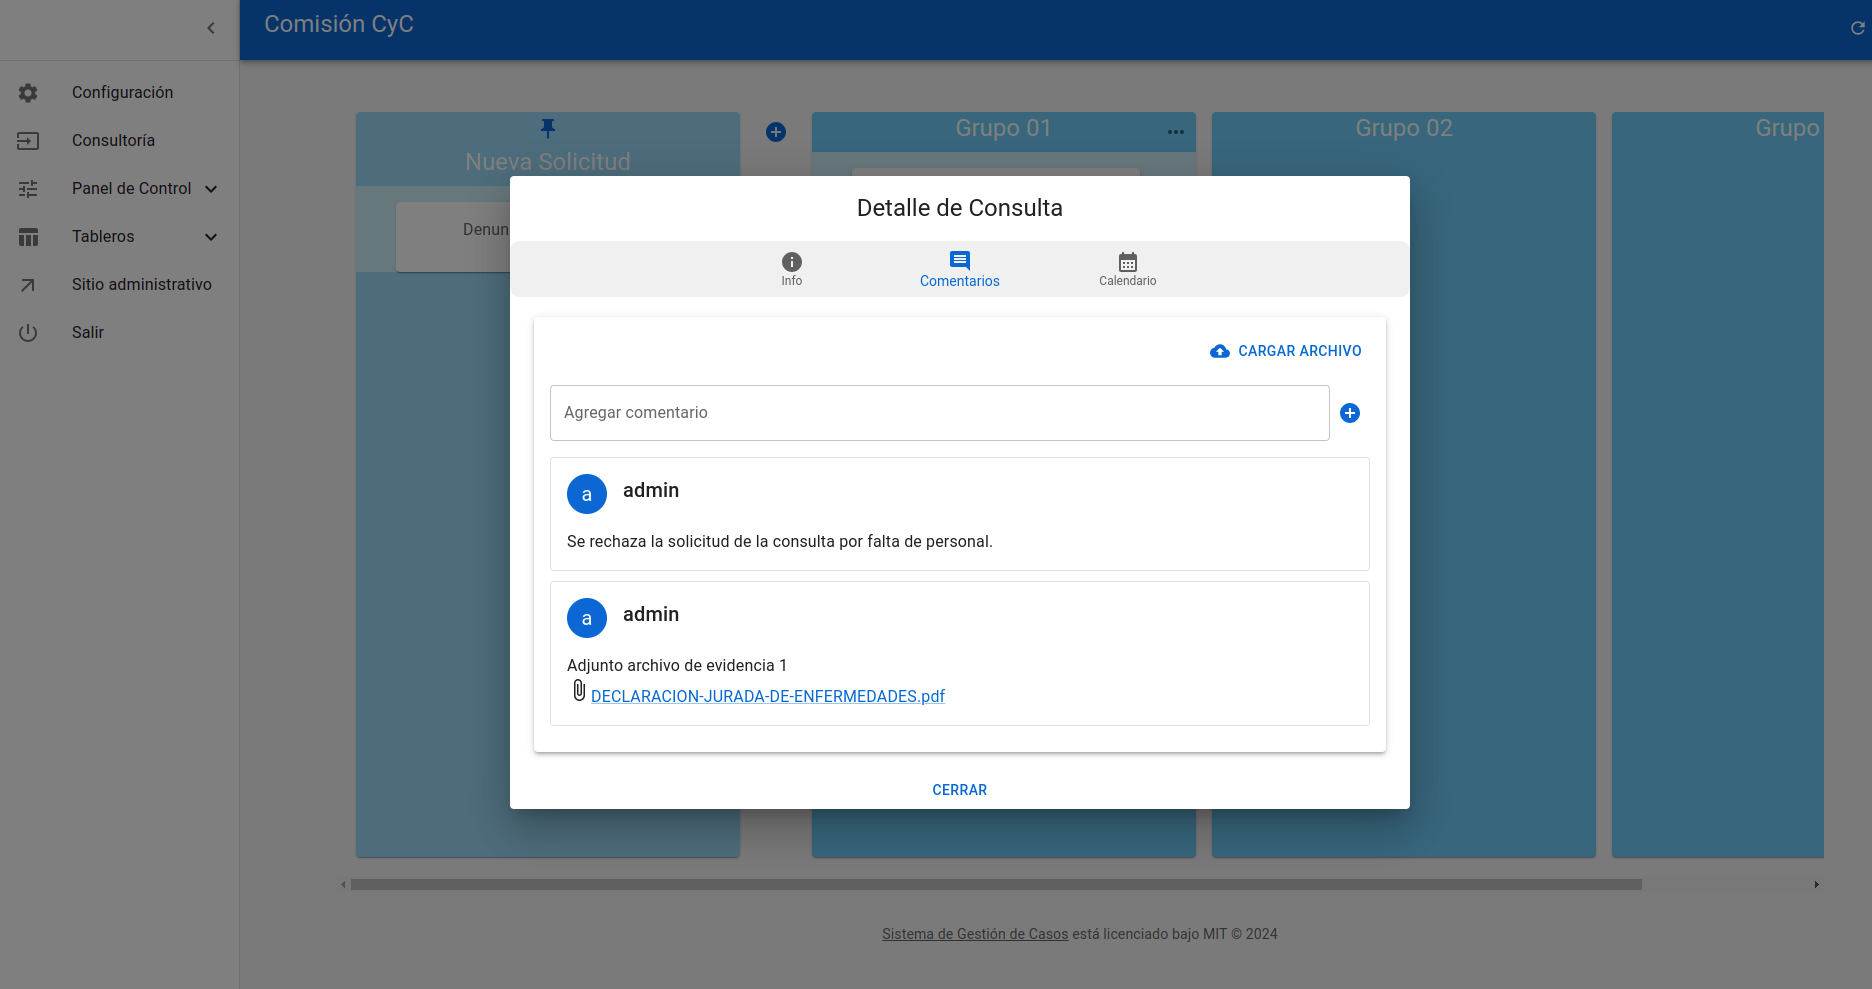
\includegraphics[width=1\linewidth]{fig/comentario-consulta.png}
    \caption{Sección de Comentarios y Archivos.}
    \label{fig:consulta-comentarios}
\end{figure}

En la figura \ref{fig:consulta-calendar-1}, muestra la segunda pestaña. Esta es una sección dedicada para registrar comentarios y archivos relevantes que contribuyan al seguimiento del caso.

\begin{figure}[H]
    \centering
    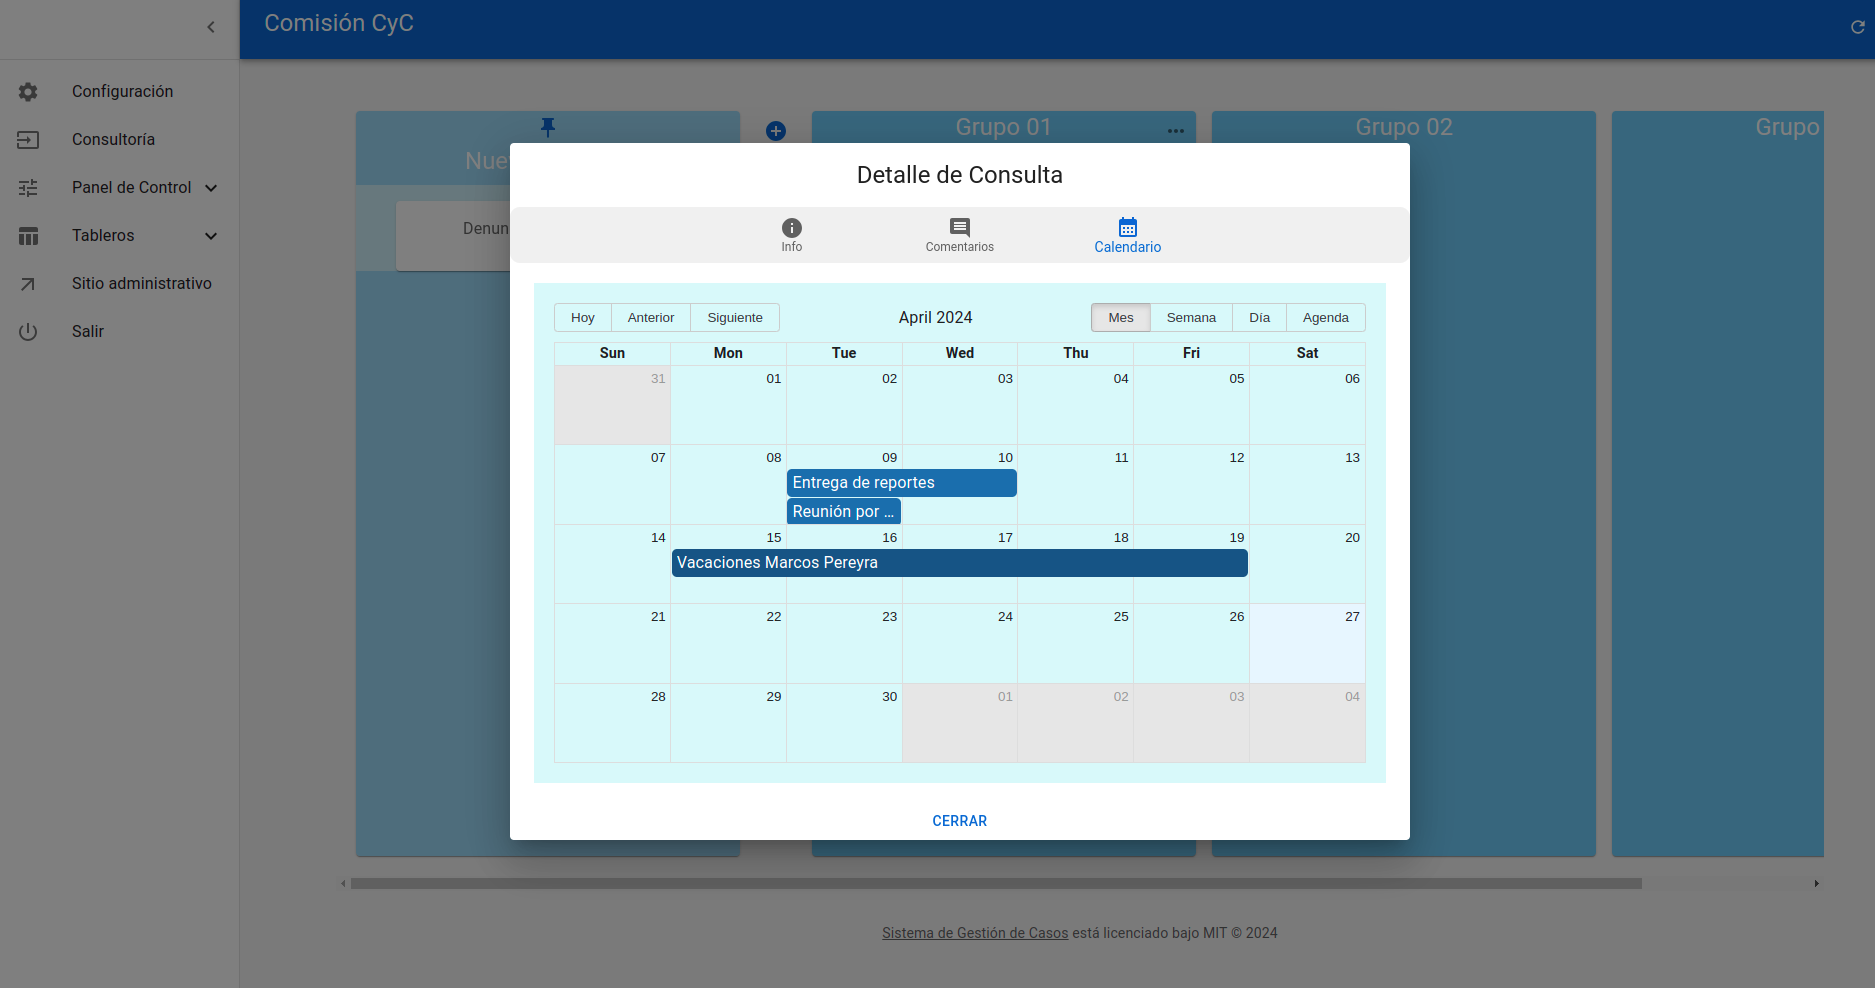
\includegraphics[width=1\linewidth]{fig/consulta-calendar-1.png}
    \caption{Calendario de Consulta.}
    \label{fig:consulta-calendar-1}
\end{figure}

En las figuras \ref{fig:consulta-calendar-2} y \ref{fig:consulta-calendar-3}, se observa la tercera ventana, que es un calendario que permite registrar eventos relacionados con el caso, como reuniones o fechas importantes.

\begin{figure}[H]
    \centering
    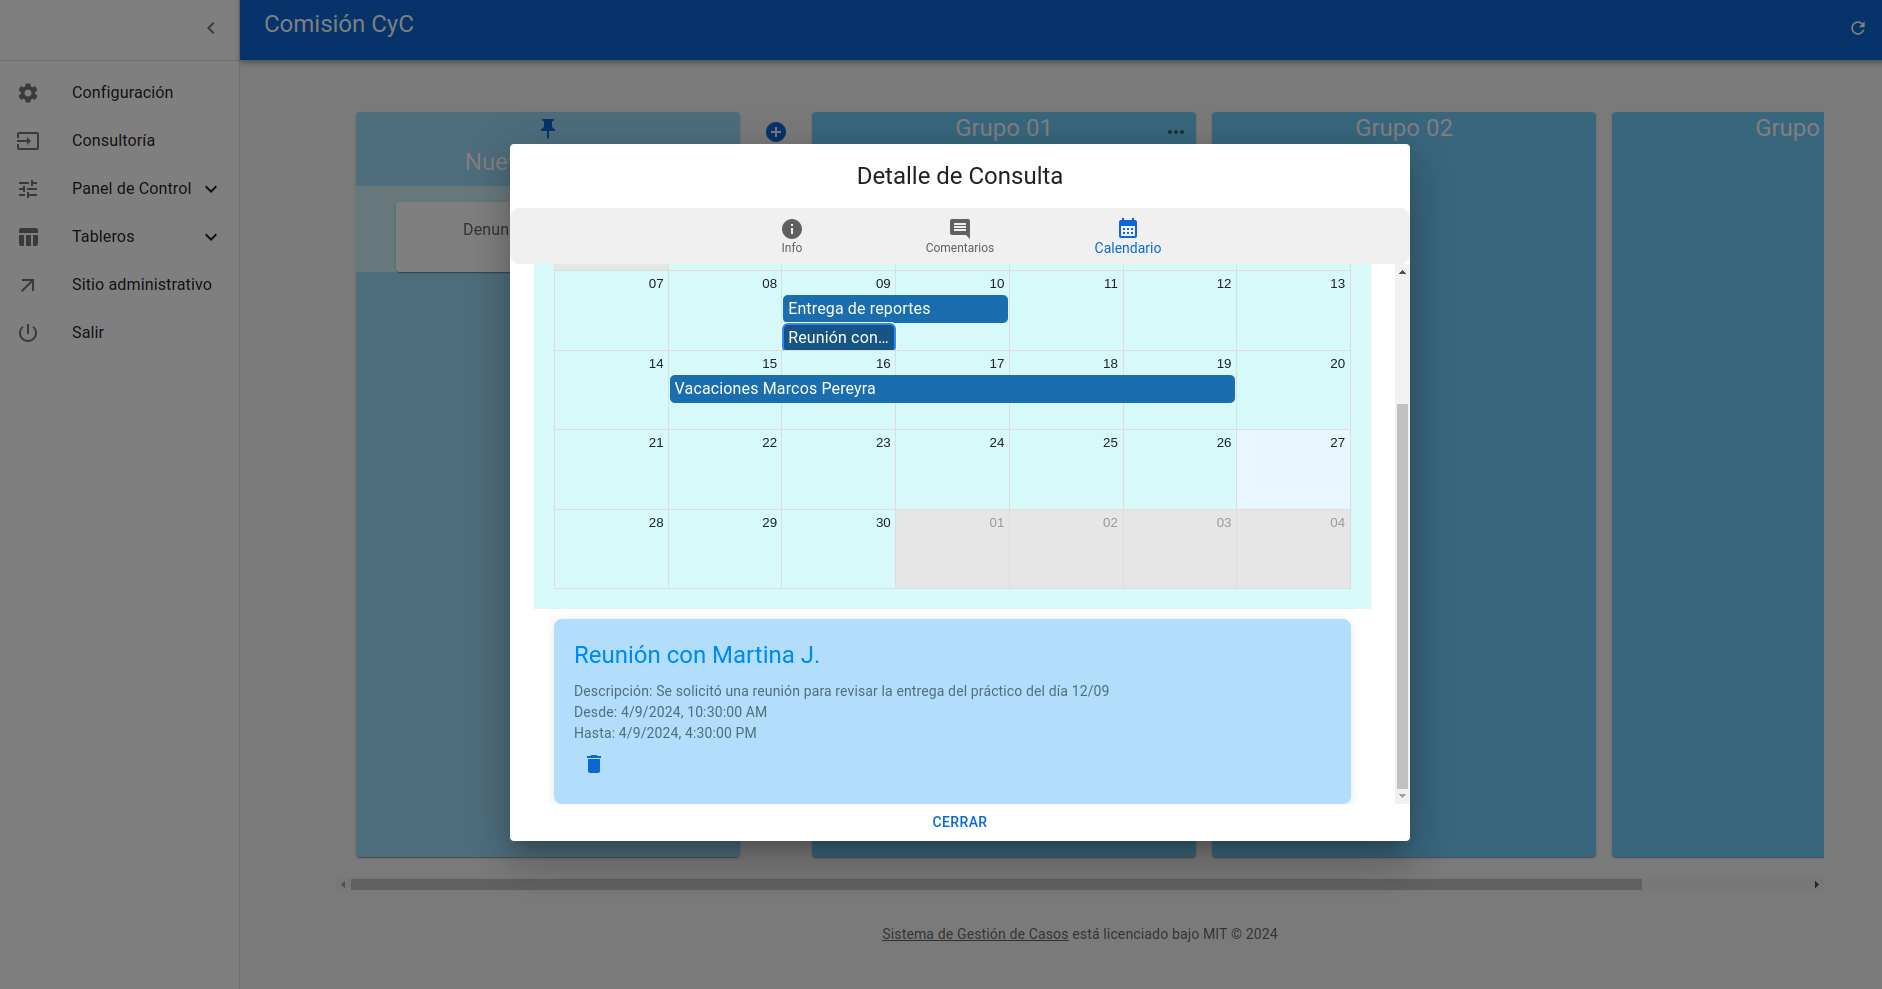
\includegraphics[width=1\linewidth]{fig/consulta-calendar-2.png}
    \caption{Detalle de Evento del Calendario de Consulta.}
    \label{fig:consulta-calendar-2}
\end{figure}
Al seleccionar un evento en el calendario, se desplegará una vista detallada con información adicional.

\begin{figure}[H]
    \centering
    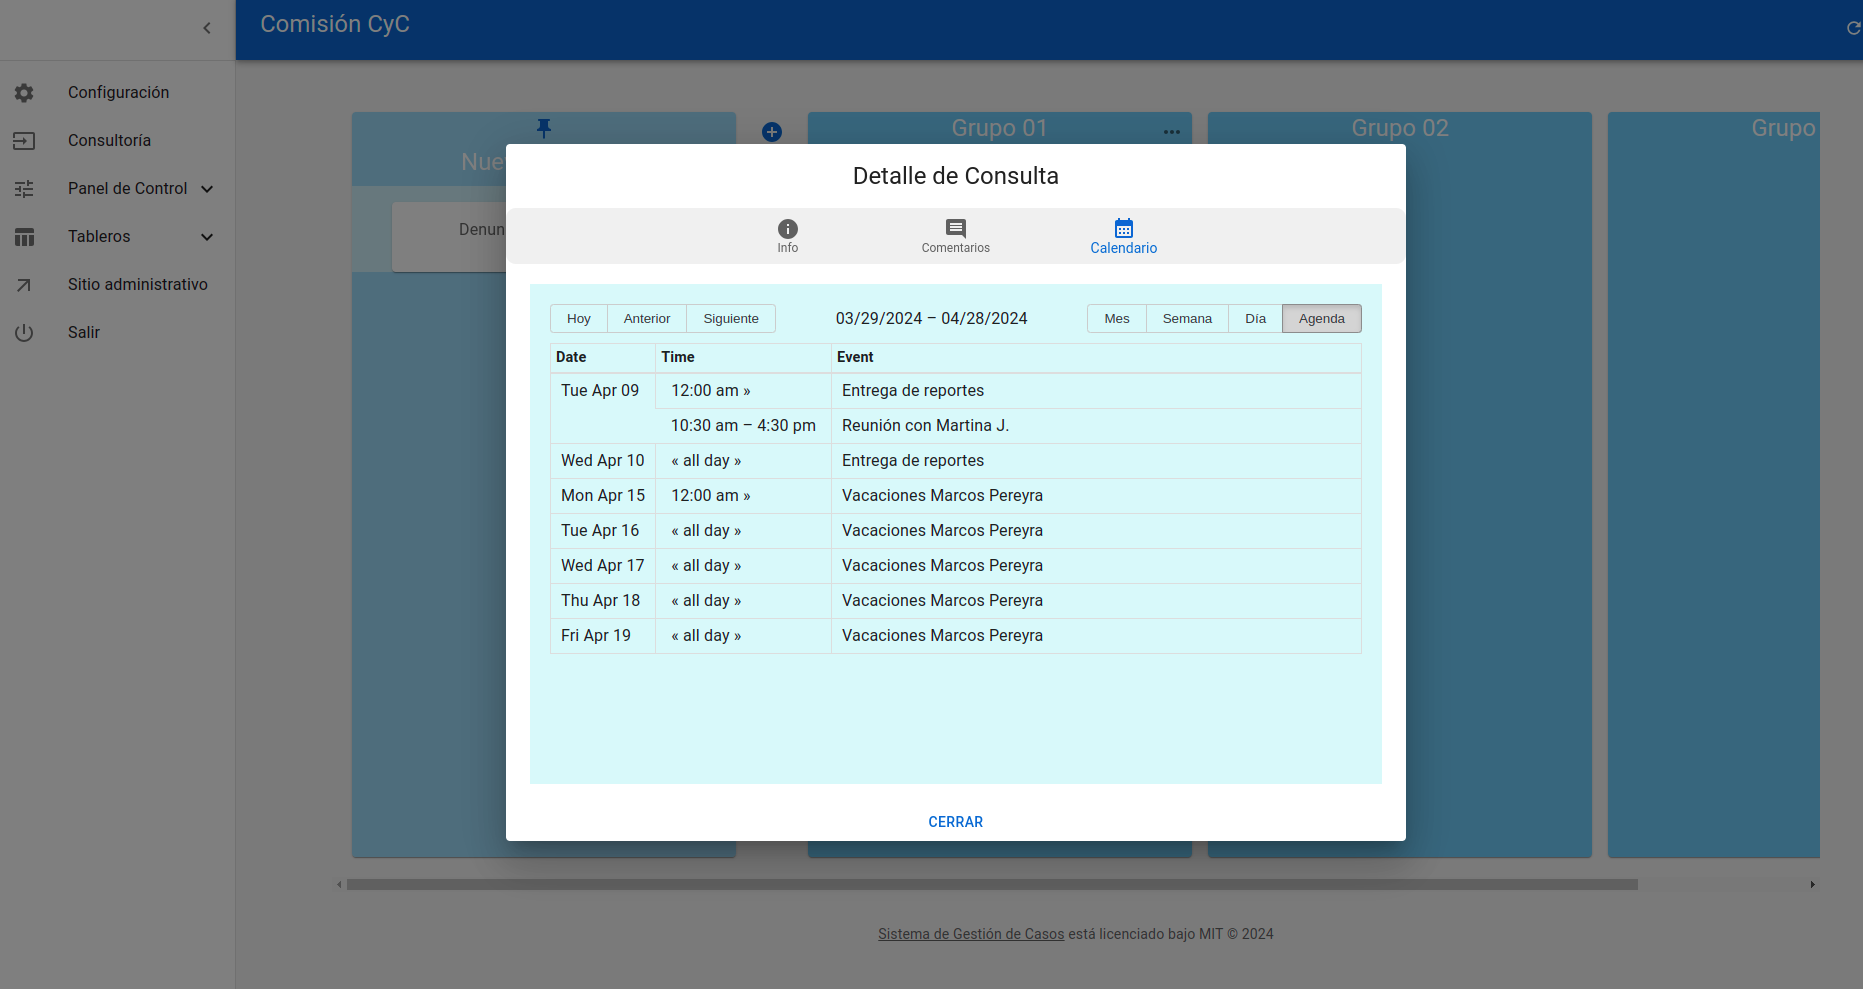
\includegraphics[width=1\linewidth]{fig/consulta-calendar-3.png}
    \caption{Vista Agenda de Calendario de Consulta.}
    \label{fig:consulta-calendar-3}
\end{figure}

Este calendario ofrece varias vistas, como mensual, semanal, diaria o en formato de agenda, según se visualiza en la imagen anterior. Es una herramienta clave para organizar y dar seguimiento a eventos relevantes asociados a la consulta.

\section{Configuración de Cuenta}\label{sec:configuracion-cuenta}

La sección de configuración de cuenta (ver Figura \ref{fig:settings-page}), accesible desde la página de ``Settings'', proporciona la capacidad de visualizar y editar información personalizada, como el nombre de usuario y la contraseña.

\begin{figure}[H]
    \centering
    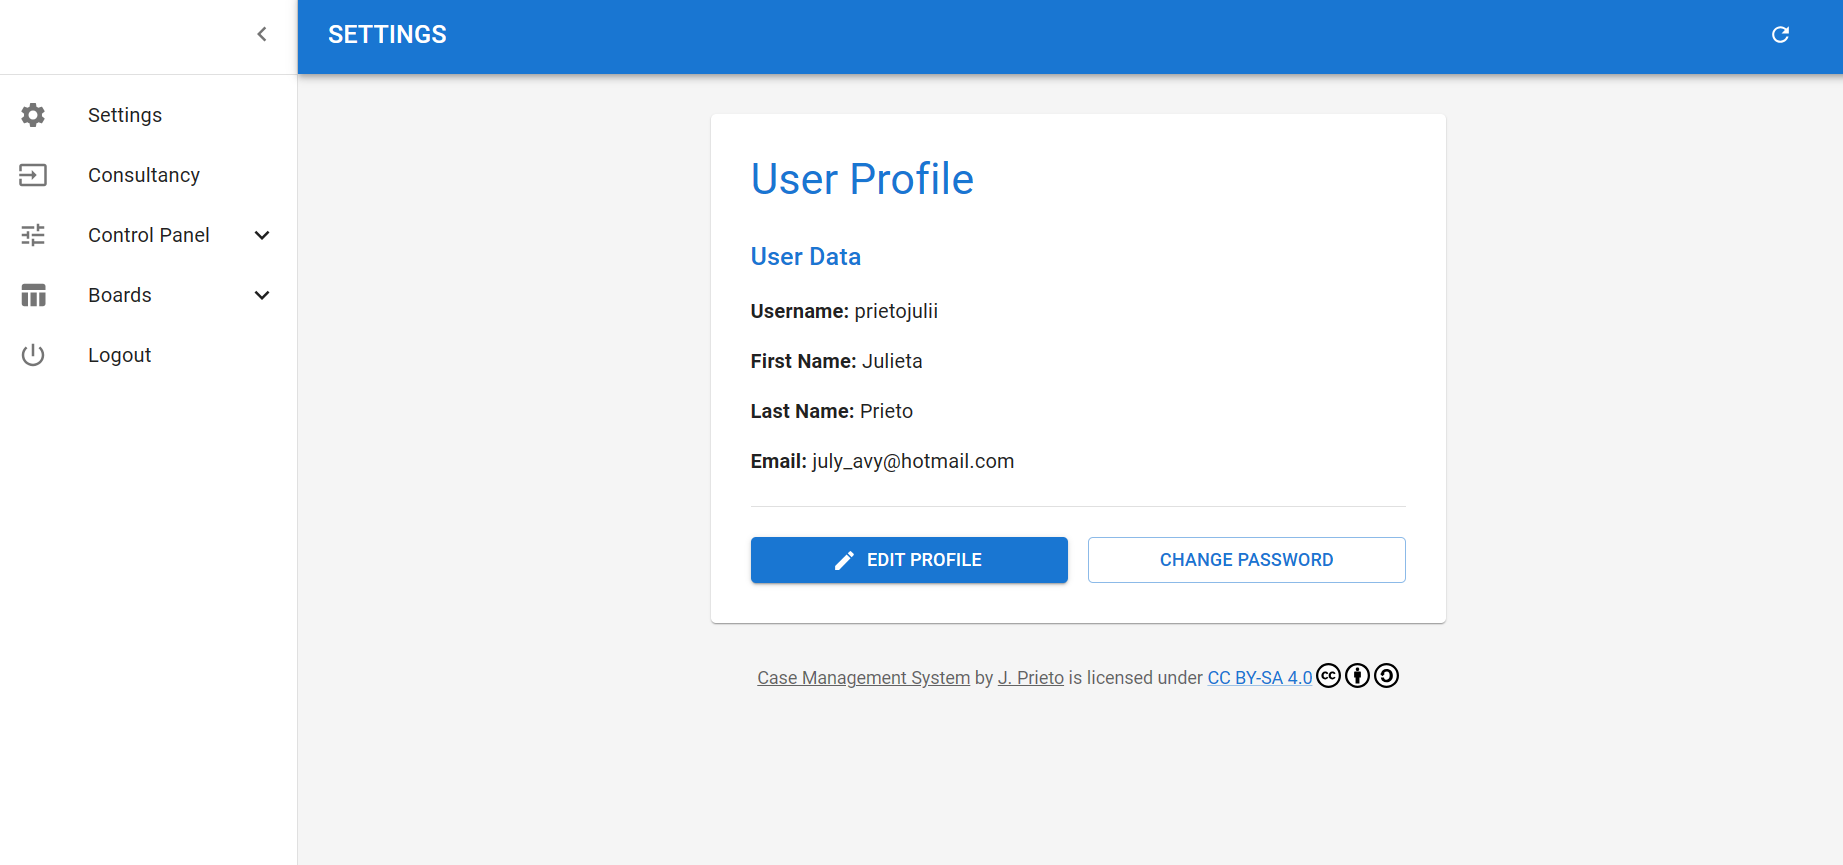
\includegraphics[width=1\linewidth]{fig/settings-real-page.png}
    \caption{Página de Configuración de Cuenta.}
    \label{fig:settings-page}
\end{figure}
